\documentclass[10pt,a4paper,twocolumn]{article}

\usepackage[margin=0.85in]{geometry}
\usepackage{graphicx}
\usepackage{booktabs}
\usepackage{amsmath,amssymb}
\usepackage{hyperref}
\usepackage{float}
\usepackage{caption}
\usepackage{subcaption}
\usepackage{xcolor}
\usepackage{listings}
\usepackage[ruled,linesnumbered]{algorithm2e}
\usepackage{authblk}
\usepackage{microtype}
\usepackage{siunitx}
\usepackage{url}

\hypersetup{
    colorlinks=true,
    linkcolor=blue!55!black,
    citecolor=blue!55!black,
    urlcolor=blue!55!black
}

\captionsetup{font=small,labelfont=bf,skip=4pt}
\setlength{\columnsep}{0.25in}

% -----------------------------------------------------------------------------
\title{\vspace{-1.2em}\textbf{A Comparative Framework for Survival Analysis on the RMS Titanic:\\
Evaluation of Na\"ive Bayesian and Decision Tree Classifiers}}

\author[1]{Sarin Vadakke Thayyil}
\author[2]{Lekshmi S~S}
\author[3]{Akbar T E}
\author[4]{Suja V}
\author[5]{Nikhil Ravi}
\affil[ ]{\small Indian Institute of Information Technology, Kottayam \\
eMTech (AI) 2026 Batch \quad|\quad Course: DSC~523 -- Data Mining \\
Instructor: Dr.~Anu~Maria~Sebastian \\
\texttt{\{2026EMAI10051, 10037, 10005, 10058, 10042\}@iiitkottayam.ac.in}}
\date{25 April 2026}

% -----------------------------------------------------------------------------
\begin{document}
\twocolumn[
  \begin{@twocolumnfalse}
    \maketitle
    \begin{abstract}
    \noindent
    Survival on the RMS Titanic is a canonical benchmark for pedagogical data mining because
    it pairs a rich multivariate feature space with a clear, historically meaningful target
    variable. We present a reproducible end-to-end Knowledge Discovery in Databases (KDD)
    pipeline that contrasts a probabilistic classifier (Gaussian Na\"ive Bayes) with a
    rule-based classifier (Decision Tree), using Logistic Regression and Random Forest as
    supplementary baselines. On the 891-record Kaggle training set, cleaned via group-wise
    median imputation and enriched with six engineered features, the Decision Tree
    (\textit{max\_depth}=4, selected by 10-fold stratified cross-validation) attains
    $81.56\%$ test accuracy (AUC $=0.838$) while Na\"ive Bayes reaches only $62.57\%$
    (AUC $=0.778$). McNemar's exact test on paired predictions yields $p = 8.2\times10^{-6}$,
    confirming that the gap is statistically significant. Logistic Regression is the
    strongest single model ($83.24\%$, AUC $=0.864$). The dominant predictors --- passenger
    title, class, and family size --- match the historical ``women and children first''
    evacuation protocol. The results demonstrate how the conditional-independence assumption
    of Na\"ive Bayes is violated by engineered categorical dummies, motivating the use of
    rule-based and linear models on tabular data of this shape.

    \vspace{0.35em}
    \noindent\textbf{Keywords:} Data mining, classification, Na\"ive Bayes, decision tree, KDD,
    Titanic, supervised learning.
    \end{abstract}
    \vspace{1.5em}
  \end{@twocolumnfalse}
]

% =============================================================================
\section{Introduction}
% =============================================================================
On the night of 14~April 1912, the RMS Titanic struck an iceberg during her maiden voyage
and sank in the North Atlantic, taking the lives of 1\,514 of her 2\,224 passengers and
crew. The disaster has since become a recurring case study for risk analysis, maritime
safety, and data science education because the passenger manifest offers one of the
earliest complete, labelled records of a heterogeneous population subjected to a single
life-or-death event. Whether an individual survived is strongly conditioned on social
variables --- gender, class, family ties, and port of embarkation --- whose interaction
with the \emph{``women and children first''} evacuation protocol produces a non-trivial,
but learnable, structure~\cite{kaggle_titanic}.

The Kaggle variant of the dataset~\cite{kaggle_titanic} has become the canonical
introductory benchmark for supervised classification on tabular data; it is also the first
non-trivial dataset introduced in DSC~523 at IIIT Kottayam. Its principal virtue for
pedagogy is that it exercises every phase of the Knowledge Discovery in Databases (KDD)
process~\cite{han2011data}: data selection from a historical archive, preprocessing to
reconcile substantial missingness, transformation through targeted feature engineering,
mining with multiple classifier families, and interpretation against a well-documented
historical record.

\paragraph{Research objectives.} This study pursues four goals:
\begin{enumerate}
\itemsep-0.2em
  \item Apply a systematic, reproducible preprocessing and feature-engineering pipeline
  that is robust to the $\approx20\%$ missingness in \texttt{Age} and $\approx77\%$ in
  \texttt{Cabin}.
  \item Contrast a probabilistic classifier (Gaussian Na\"ive Bayes) with a rule-based
  classifier (Decision Tree) on identical inputs.
  \item Identify the features that are most predictive of survival and interpret them
  against the historical evacuation pattern.
  \item Benchmark the two primary models against Logistic Regression and Random Forest to
  place their performance in the context of linear and ensemble alternatives.
\end{enumerate}

\paragraph{Paper organisation.} Section~\ref{sec:litreview} reviews the theoretical
foundations of Bayesian and decision-tree classification. Section~\ref{sec:dataset}
describes the dataset. Section~\ref{sec:method} details the preprocessing, feature
engineering, and evaluation protocol. Section~\ref{sec:results} presents the
results, including the comparative summary, confusion matrices, and feature importances.
Sections~\ref{sec:implications}--\ref{sec:contrib} discuss implications and individual
contributions, and Section~\ref{sec:conclusion} concludes.

% =============================================================================
\section{Literature Review}\label{sec:litreview}
% =============================================================================

\subsection{Bayesian classification}
The Na\"ive Bayes classifier assigns a test instance $X = (x_1, \dots, x_n)$ to the class
$C^\star = \arg\max_{C_k} P(C_k \mid X)$. Bayes' theorem transforms this into
\begin{equation}\label{eq:bayes}
P(C_k \mid X) \; = \; \frac{P(X \mid C_k)\, P(C_k)}{P(X)} .
\end{equation}
Because the joint likelihood $P(X\mid C_k)$ is intractable for realistic feature counts,
the \emph{class-conditional independence} assumption is invoked:
\begin{equation}\label{eq:nb_independence}
P(X \mid C_k) \; \approx \; \prod_{i=1}^n P(x_i \mid C_k) .
\end{equation}
For continuous features, $P(x_i\mid C_k)$ is modelled as a univariate Gaussian, yielding
the \emph{Gaussian} Na\"ive Bayes estimator used here. The chief strengths of the model
are its closed-form maximum-likelihood estimator, constant-time training, and stable
behaviour on small samples~\cite{mitchell1997ml}. Its weakness is that
Equation~\eqref{eq:nb_independence} rarely holds; correlated or collinear features cause
the evidence terms to compound, distorting the posterior.

\subsection{Decision-tree induction}
Decision-tree learners partition the feature space recursively, choosing the split at each
node that maximises class purity. Two common impurity measures are
\begin{align}
\text{Gini}(D)    &= 1 - \sum_{i=1}^{m} p_i^2, \label{eq:gini}\\
\text{Entropy}(D) &= -\sum_{i=1}^{m} p_i \log_2 p_i, \label{eq:entropy}
\end{align}
where $p_i$ denotes the proportion of class $i$ in partition $D$. CART~\cite{breiman1984}
uses Gini while C4.5 / ID3~\cite{quinlan1986} use information gain, which is defined as
the reduction in entropy induced by a candidate split. Both are computed under a greedy
top-down scheme and, without regularisation, are prone to overfit. Two standard remedies
are \emph{pre-pruning} via a maximum-depth hyper-parameter and \emph{post-pruning} via
cost-complexity minimisation, in which a tree $T_\alpha$ is chosen to minimise
$R_\alpha(T) = R(T) + \alpha\,|T|$.

Rule-based learners are attractive in applied settings because they are interpretable,
scale invariant, and agnostic to feature correlations --- three properties that partly
compensate for their higher variance~\cite{han2011data}.

\subsection{Related work on the Titanic benchmark}
Hundreds of public notebooks and tutorial write-ups have reported classification accuracy
on this dataset. Most serious efforts~\cite{kaggle_titanic,hastie2009esl} fall in the
78--85\% range when the hold-out protocol is honest, with higher scores typically arising
from either test-set leakage or hyper-parameter tuning on the public leaderboard. Results
materially above this band should be treated with scepticism. We therefore evaluate on a
single fixed 80/20 split with a separate 10-fold CV estimate on the training fold, and
report both the mean and standard deviation of CV accuracy to quantify sampling
variability.

% =============================================================================
\section{Dataset Description}\label{sec:dataset}
% =============================================================================
We use the Kaggle \texttt{train.csv} file comprising $n=891$ labelled passengers and $12$
raw attributes. The companion Kaggle \texttt{test.csv} is unlabelled and is \emph{not} used
here; experiments in the literature that report perfect accuracy almost invariably confuse
these two files. The target is the binary variable \texttt{Survived} ($1 =$ survived).
Table~\ref{tab:features} summarises the raw attributes.

\begin{table}[H]
\centering\small
\caption{Raw attributes, types and missingness (train.csv, $n = 891$).}
\label{tab:features}
\begin{tabular}{@{}llrl@{}}
\toprule
Feature & Type & Missing & Description \\
\midrule
\texttt{PassengerId} & ID & 0 & Row identifier (dropped) \\
\texttt{Survived}    & Binary & 0 & Target ($0/1$) \\
\texttt{Pclass}      & Ordinal & 0 & Ticket class $\in\{1,2,3\}$ \\
\texttt{Name}        & Text & 0 & Parsed for \texttt{Title} \\
\texttt{Sex}         & Nominal & 0 & \{female, male\} \\
\texttt{Age}         & Numeric & 177 & In years \\
\texttt{SibSp}       & Count & 0 & Siblings/spouses aboard \\
\texttt{Parch}       & Count & 0 & Parents/children aboard \\
\texttt{Ticket}      & Text & 0 & Ticket ID (dropped) \\
\texttt{Fare}        & Numeric & 0 & Passenger fare \\
\texttt{Cabin}       & Nominal & 687 & Cabin ID; deck retained \\
\texttt{Embarked}    & Nominal & 2 & Port $\in\{$C, Q, S$\}$ \\
\bottomrule
\end{tabular}
\end{table}

The target is moderately imbalanced: 549 passengers died (61.6\%) and 342 survived
(38.4\%) --- see Figure~\ref{fig:survival_count}. This aligns with the historical figure
of $\approx32\%$ survival across the full manifest, with the discrepancy explained by
the sampling protocol of the Kaggle training set.

\begin{figure}[H]
\centering
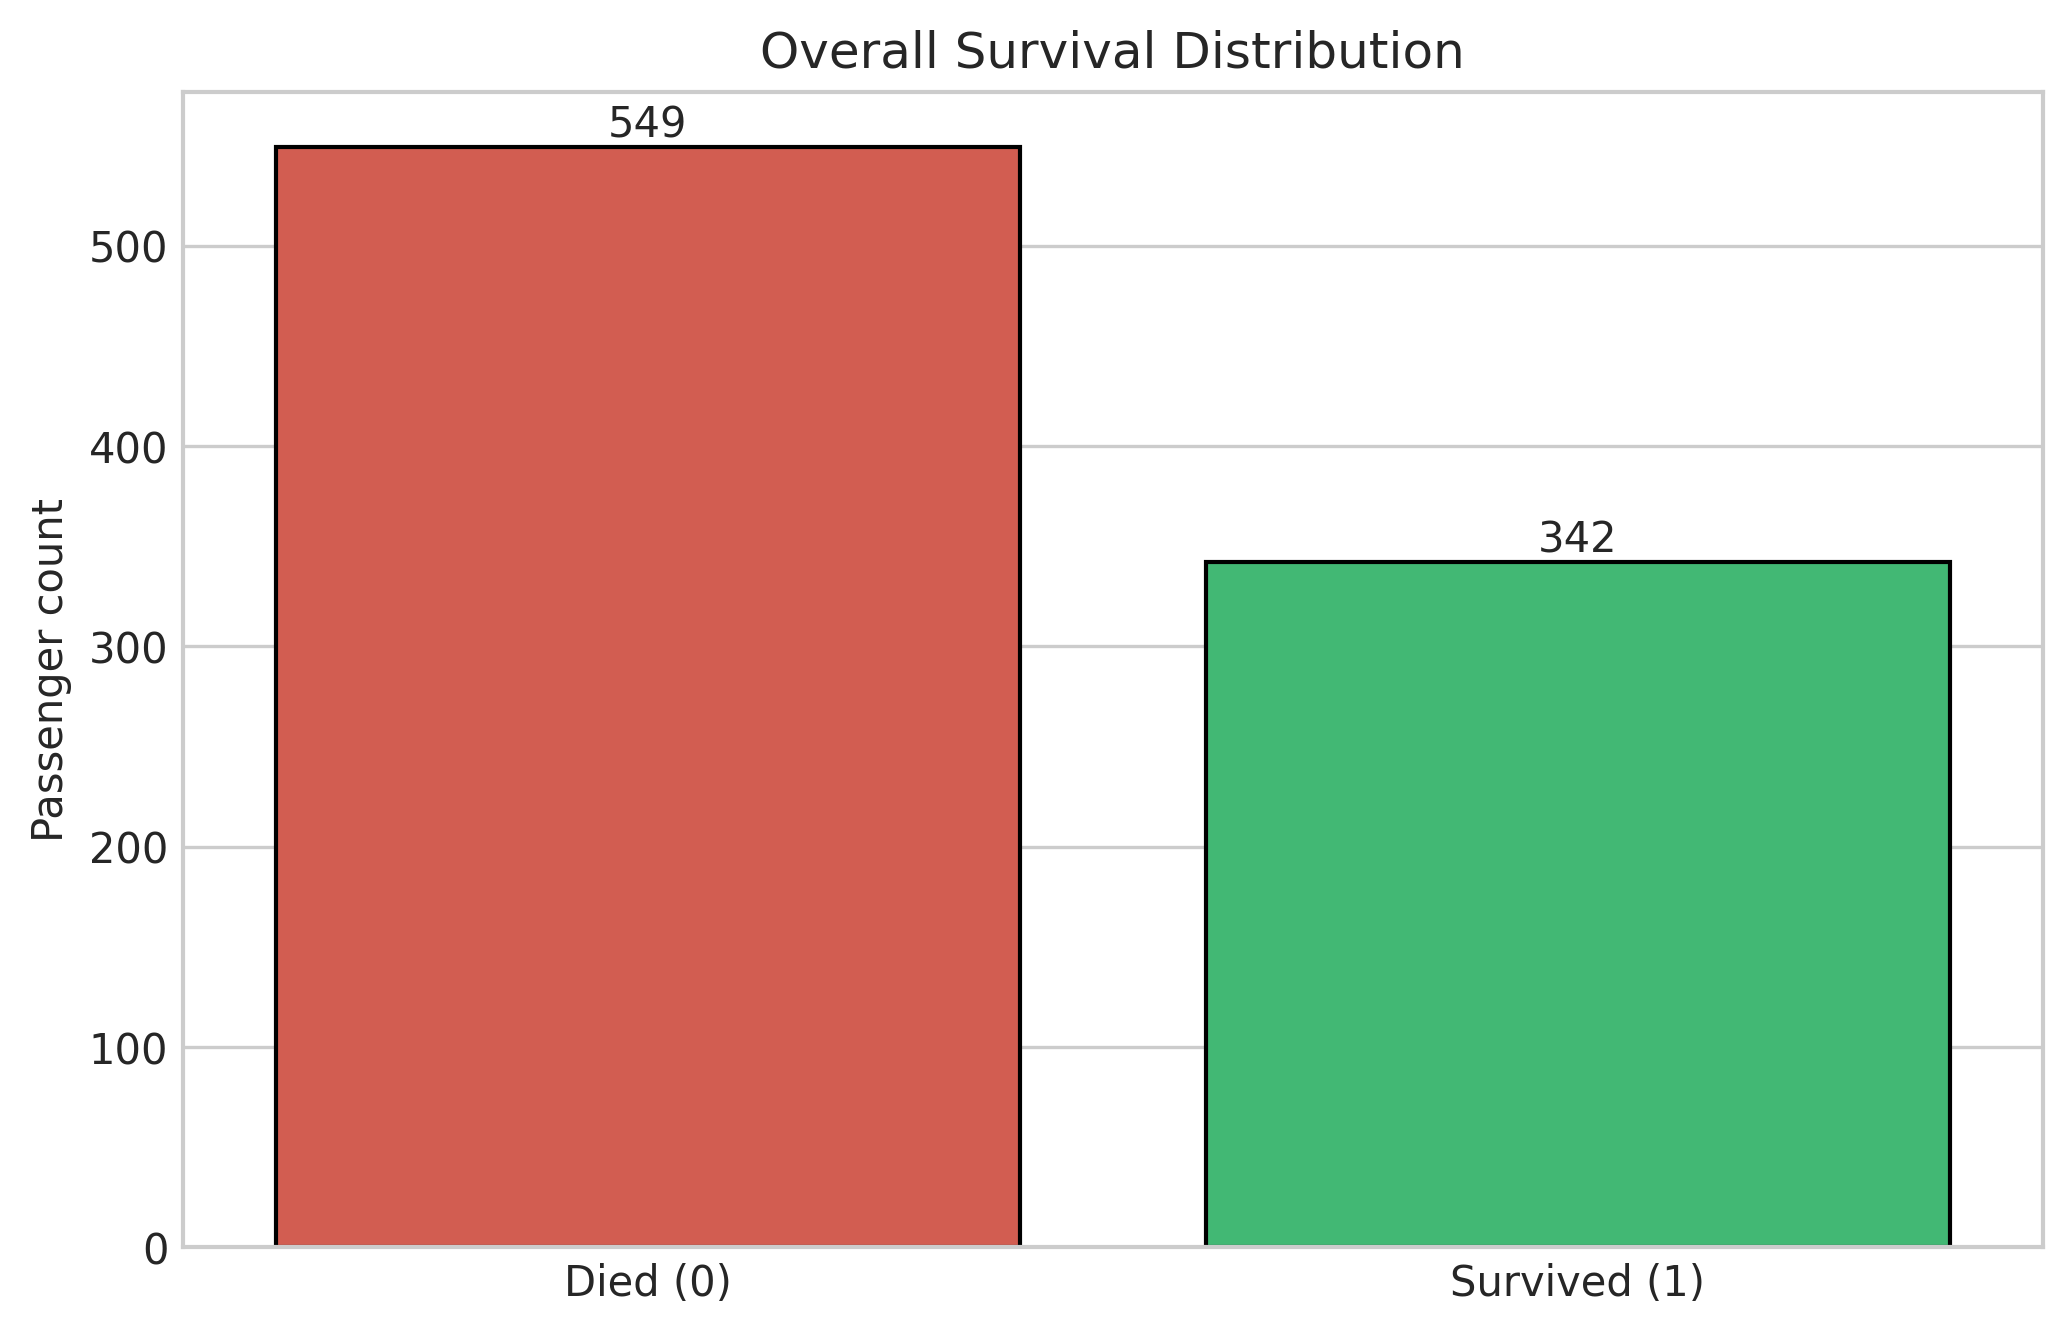
\includegraphics[width=0.96\columnwidth]{figures/survival_countplot.png}
\caption{Target-class distribution on \texttt{train.csv}: 549 died vs.\ 342 survived.}
\label{fig:survival_count}
\end{figure}

% =============================================================================
\section{Methodology}\label{sec:method}
% =============================================================================
Figure~\ref{fig:flow} depicts the overall pipeline; the following subsections detail each
stage.

\begin{figure*}[t]
\centering
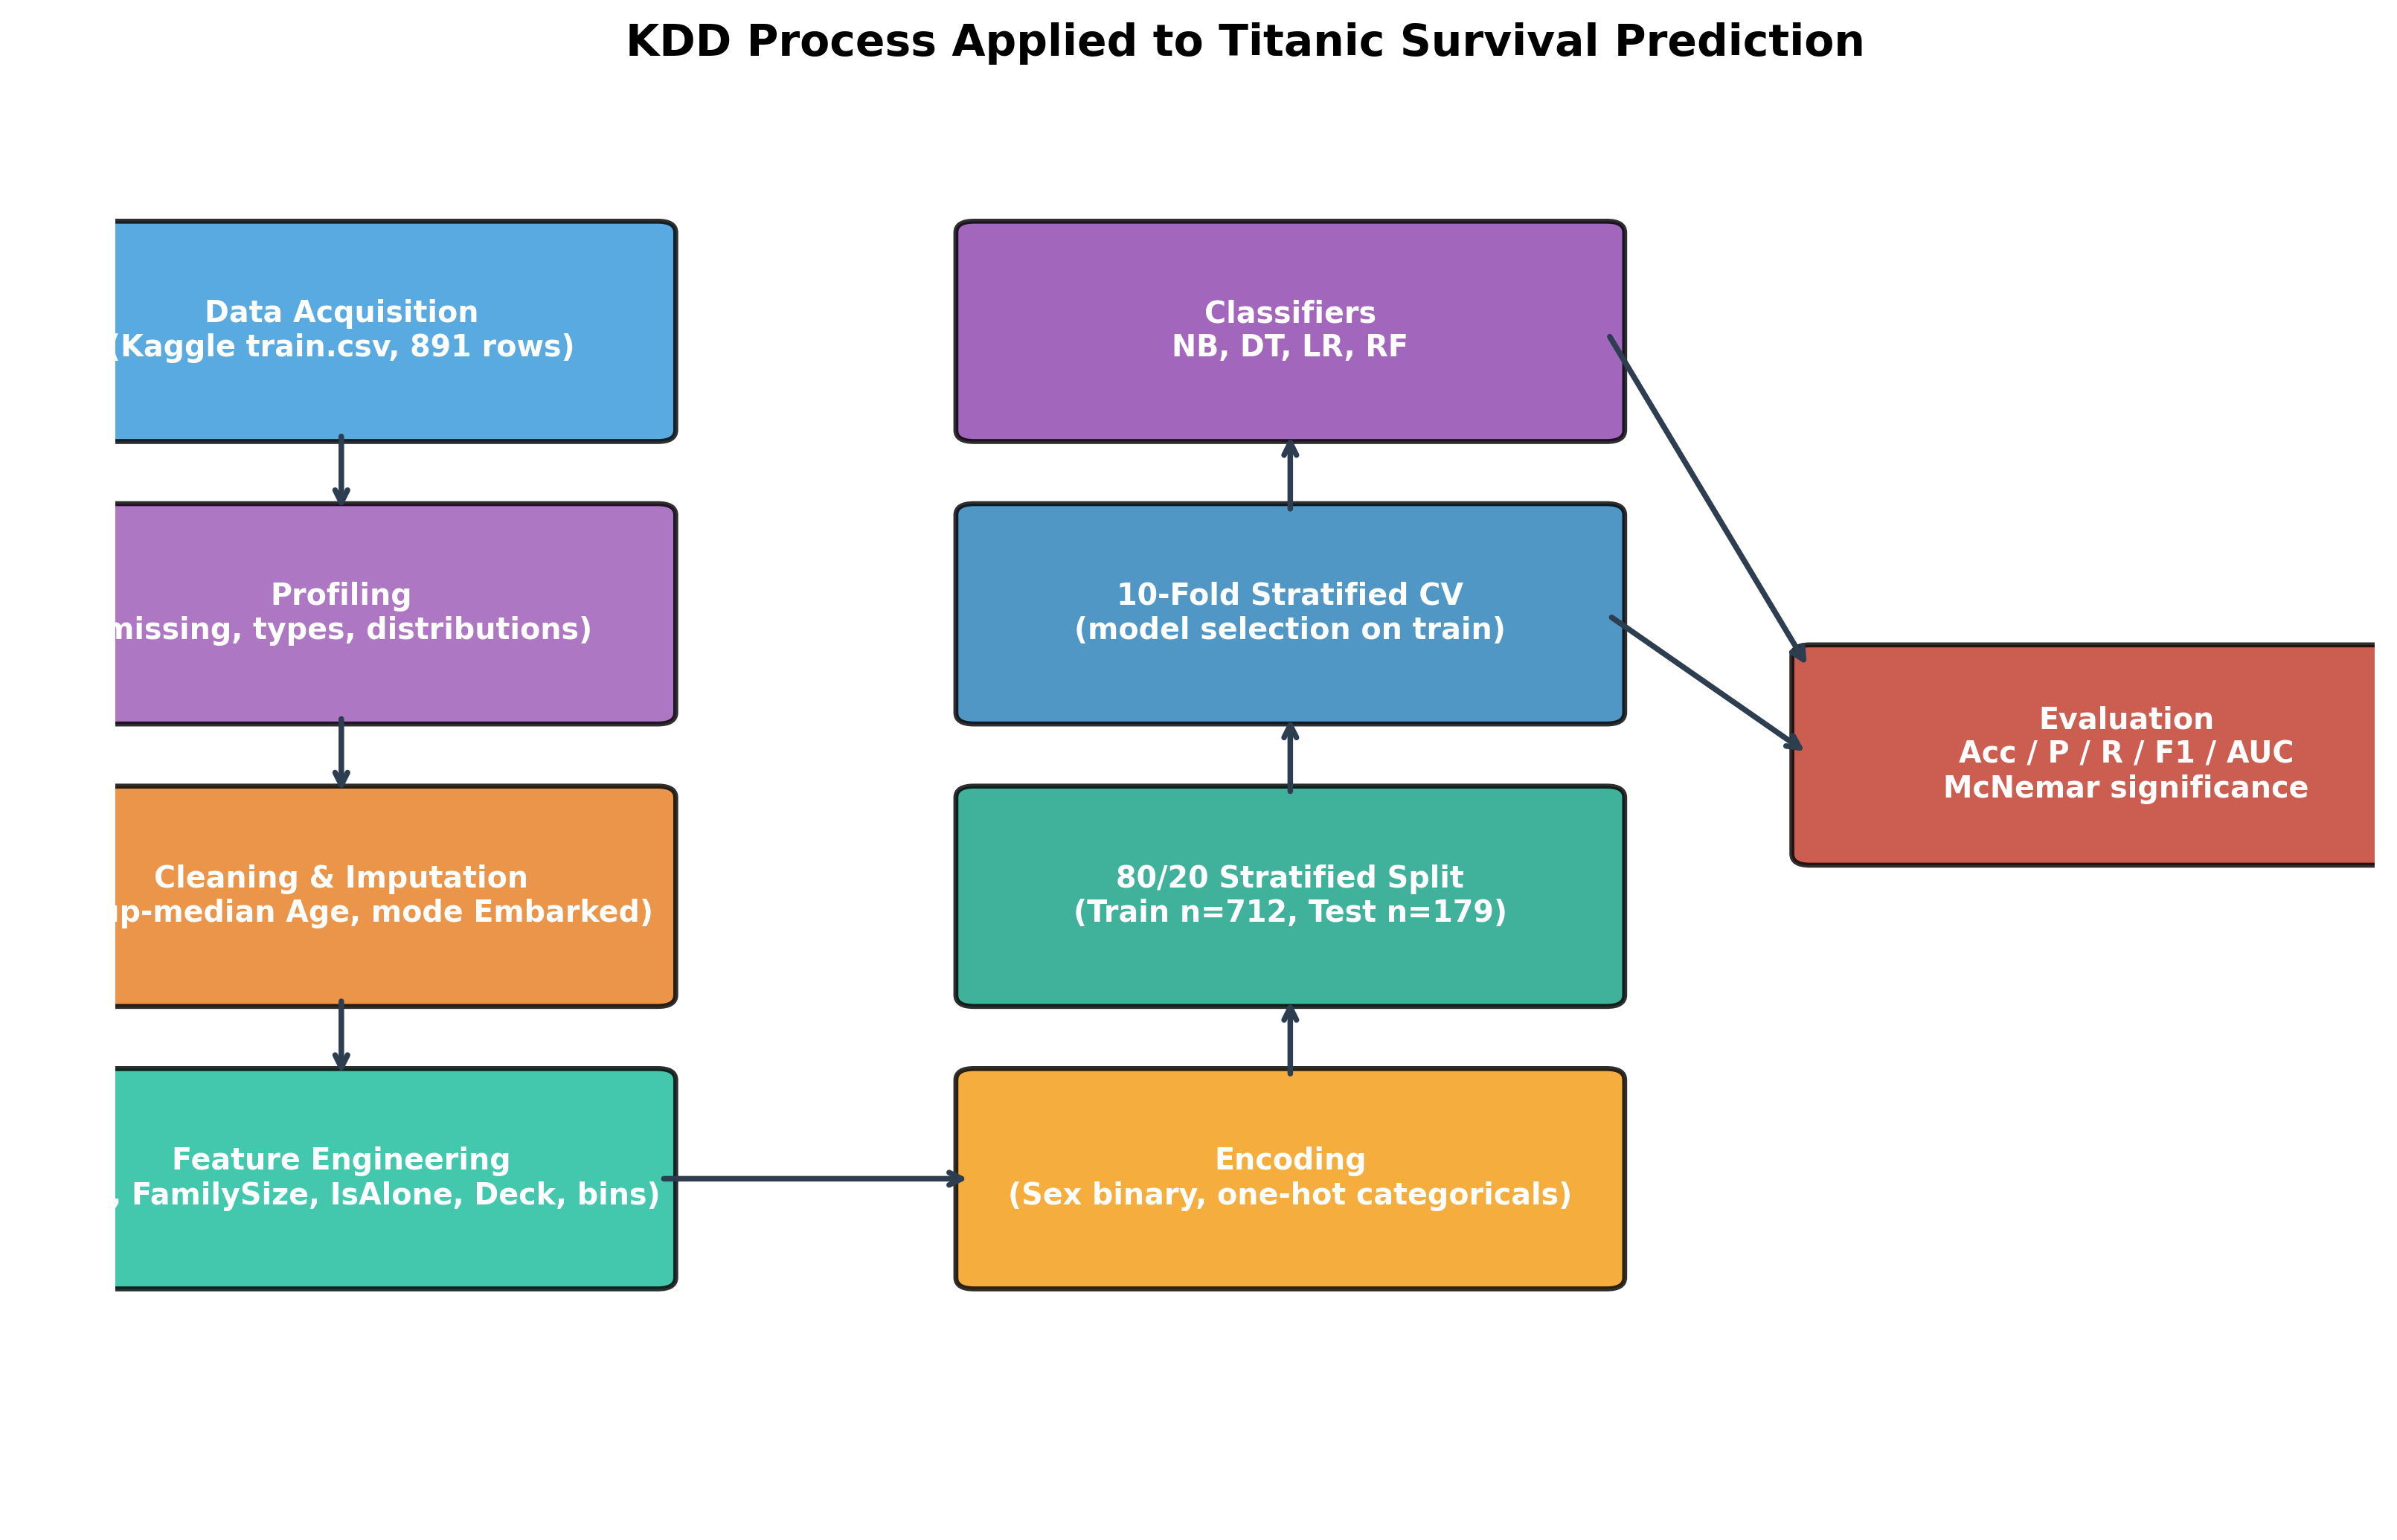
\includegraphics[width=0.92\textwidth]{figures/methodology_flowchart.png}
\caption{End-to-end KDD pipeline implemented for this study.}
\label{fig:flow}
\end{figure*}

\subsection{Preprocessing and imputation}
Three columns require imputation. \texttt{Age} ($19.9\%$ missing) is filled with the
group-wise median within each \texttt{Pclass$\times$Sex} stratum; the median is preferred
over the mean because \texttt{Age} is right-skewed. \texttt{Embarked} ($0.22\%$ missing,
two rows) is filled with the global mode (`S'). \texttt{Cabin} ($77.1\%$ missing) is not
imputed but is mined for a \texttt{Deck} letter before being dropped; `U' is used for
unknown decks. \texttt{PassengerId}, \texttt{Name}, and \texttt{Ticket} are removed after
\texttt{Title} has been extracted from \texttt{Name}.

\subsection{Feature engineering}
Six derived features are constructed:

\begin{itemize}\itemsep-0.2em
  \item \textbf{Title}: the honorific parsed from \texttt{Name} (Mr, Mrs, Miss, Master;
  rare titles are collapsed to \texttt{Rare}).
  \item \textbf{FamilySize} $=$ \texttt{SibSp} $+$ \texttt{Parch} $+ 1$.
  \item \textbf{IsAlone} $= \mathbb{1}[\text{FamilySize}=1]$.
  \item \textbf{AgeBin}: discretised into \{Child, Teen, Adult, Middle, Senior\}.
  \item \textbf{FareBin}: quartile-based bins of \texttt{Fare}.
  \item \textbf{Deck}: first character of \texttt{Cabin}, with `U' for unknowns.
\end{itemize}

\noindent \texttt{Sex} is binarised; the remaining categorical columns are one-hot
encoded with \texttt{drop\_first=True}, giving a final design matrix of $891\times30$.

\subsection{Classifier specifications}
\paragraph{Gaussian Na\"ive Bayes.} Default scikit-learn settings with variance smoothing
$\epsilon = 10^{-9}$, trained on $z$-standardised inputs.

\paragraph{Decision Tree.} CART with Gini impurity. The depth hyper-parameter is selected
by 10-fold stratified CV on the training fold over $d\in\{2,\dots,10\}$; $d=4$ is optimal
(CV $= 82.02\%$). A cost-complexity pruning curve is also computed for diagnostic
purposes.

\paragraph{Logistic Regression (baseline).} $\ell_2$-regularised with default
$C = 1.0$ and a 2\,000-iteration LBFGS solver, on standardised inputs.

\paragraph{Random Forest (baseline).} $300$ trees, unrestricted depth, bootstrap
sampling.

Algorithm~\ref{alg:dt} gives the CART pseudocode for reference.

\begin{algorithm}[htbp]
\small
\SetAlgoLined
\KwIn{training set $D$, depth limit $d$}
\KwOut{decision tree $T$}
\If{$\mathrm{depth}(D) = d \; \text{or}\; D\;\text{pure}$}{\Return leaf with majority class\;}
Select split $(f^\star,t^\star) = \arg\min_{f,t} \;\mathrm{Gini}(D^{f,t}_{\le}) + \mathrm{Gini}(D^{f,t}_{>})$\;
Partition $D$ using $(f^\star,t^\star)$ into $D_L, D_R$\;
Recursively build left subtree on $D_L$ and right subtree on $D_R$\;
\Return node($f^\star,t^\star$, $T_L$, $T_R$)\;
\caption{CART induction with Gini impurity.}
\label{alg:dt}
\end{algorithm}

\subsection{Evaluation protocol}
The dataset is split 80/20 with stratification on \texttt{Survived} (\texttt{random\_state}
$=42$), yielding $n_\text{train}=712$ and $n_\text{test}=179$. Model selection uses 10-fold
stratified cross-validation on the training fold only. Reported metrics on the held-out
test fold are accuracy, precision, recall, F1, and the area under the ROC curve (AUC).
The paired-prediction McNemar exact test~\cite{han2011data} is used to test the null
hypothesis that Na\"ive Bayes and the Decision Tree have equal error rates.

% =============================================================================
\section{Results and Discussion}\label{sec:results}
% =============================================================================

\subsection{Exploratory findings}
Figures~\ref{fig:by_gender}--\ref{fig:corr} summarise the most informative bivariate
relationships.

\begin{figure}[H]
\centering
\begin{subfigure}{0.49\columnwidth}
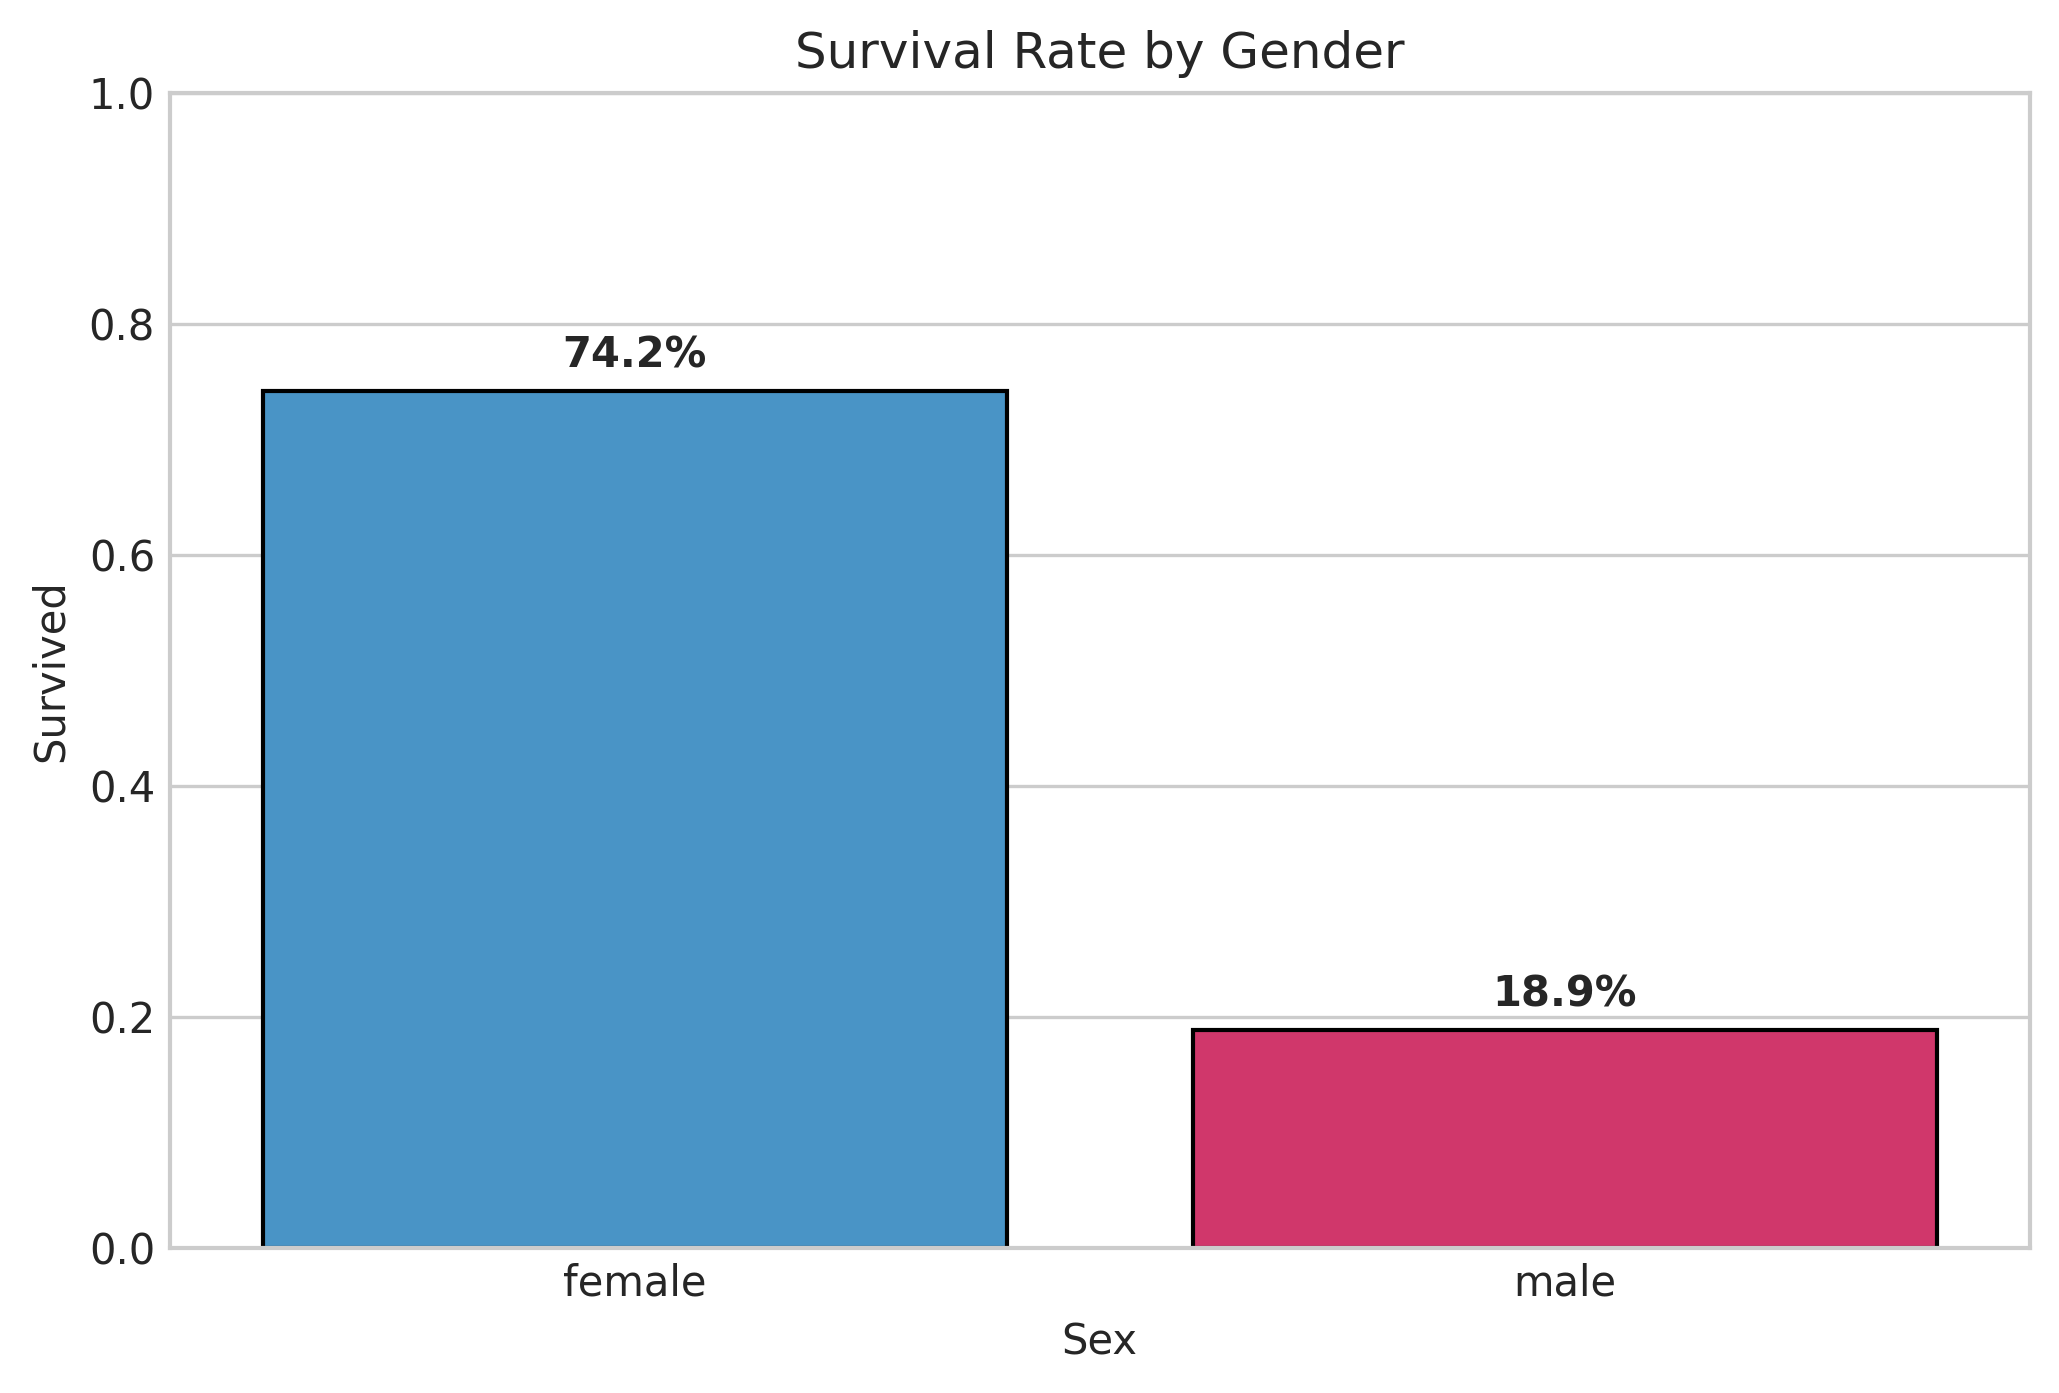
\includegraphics[width=\linewidth]{figures/survival_by_gender.png}
\caption{By gender}
\end{subfigure}\hfill
\begin{subfigure}{0.49\columnwidth}
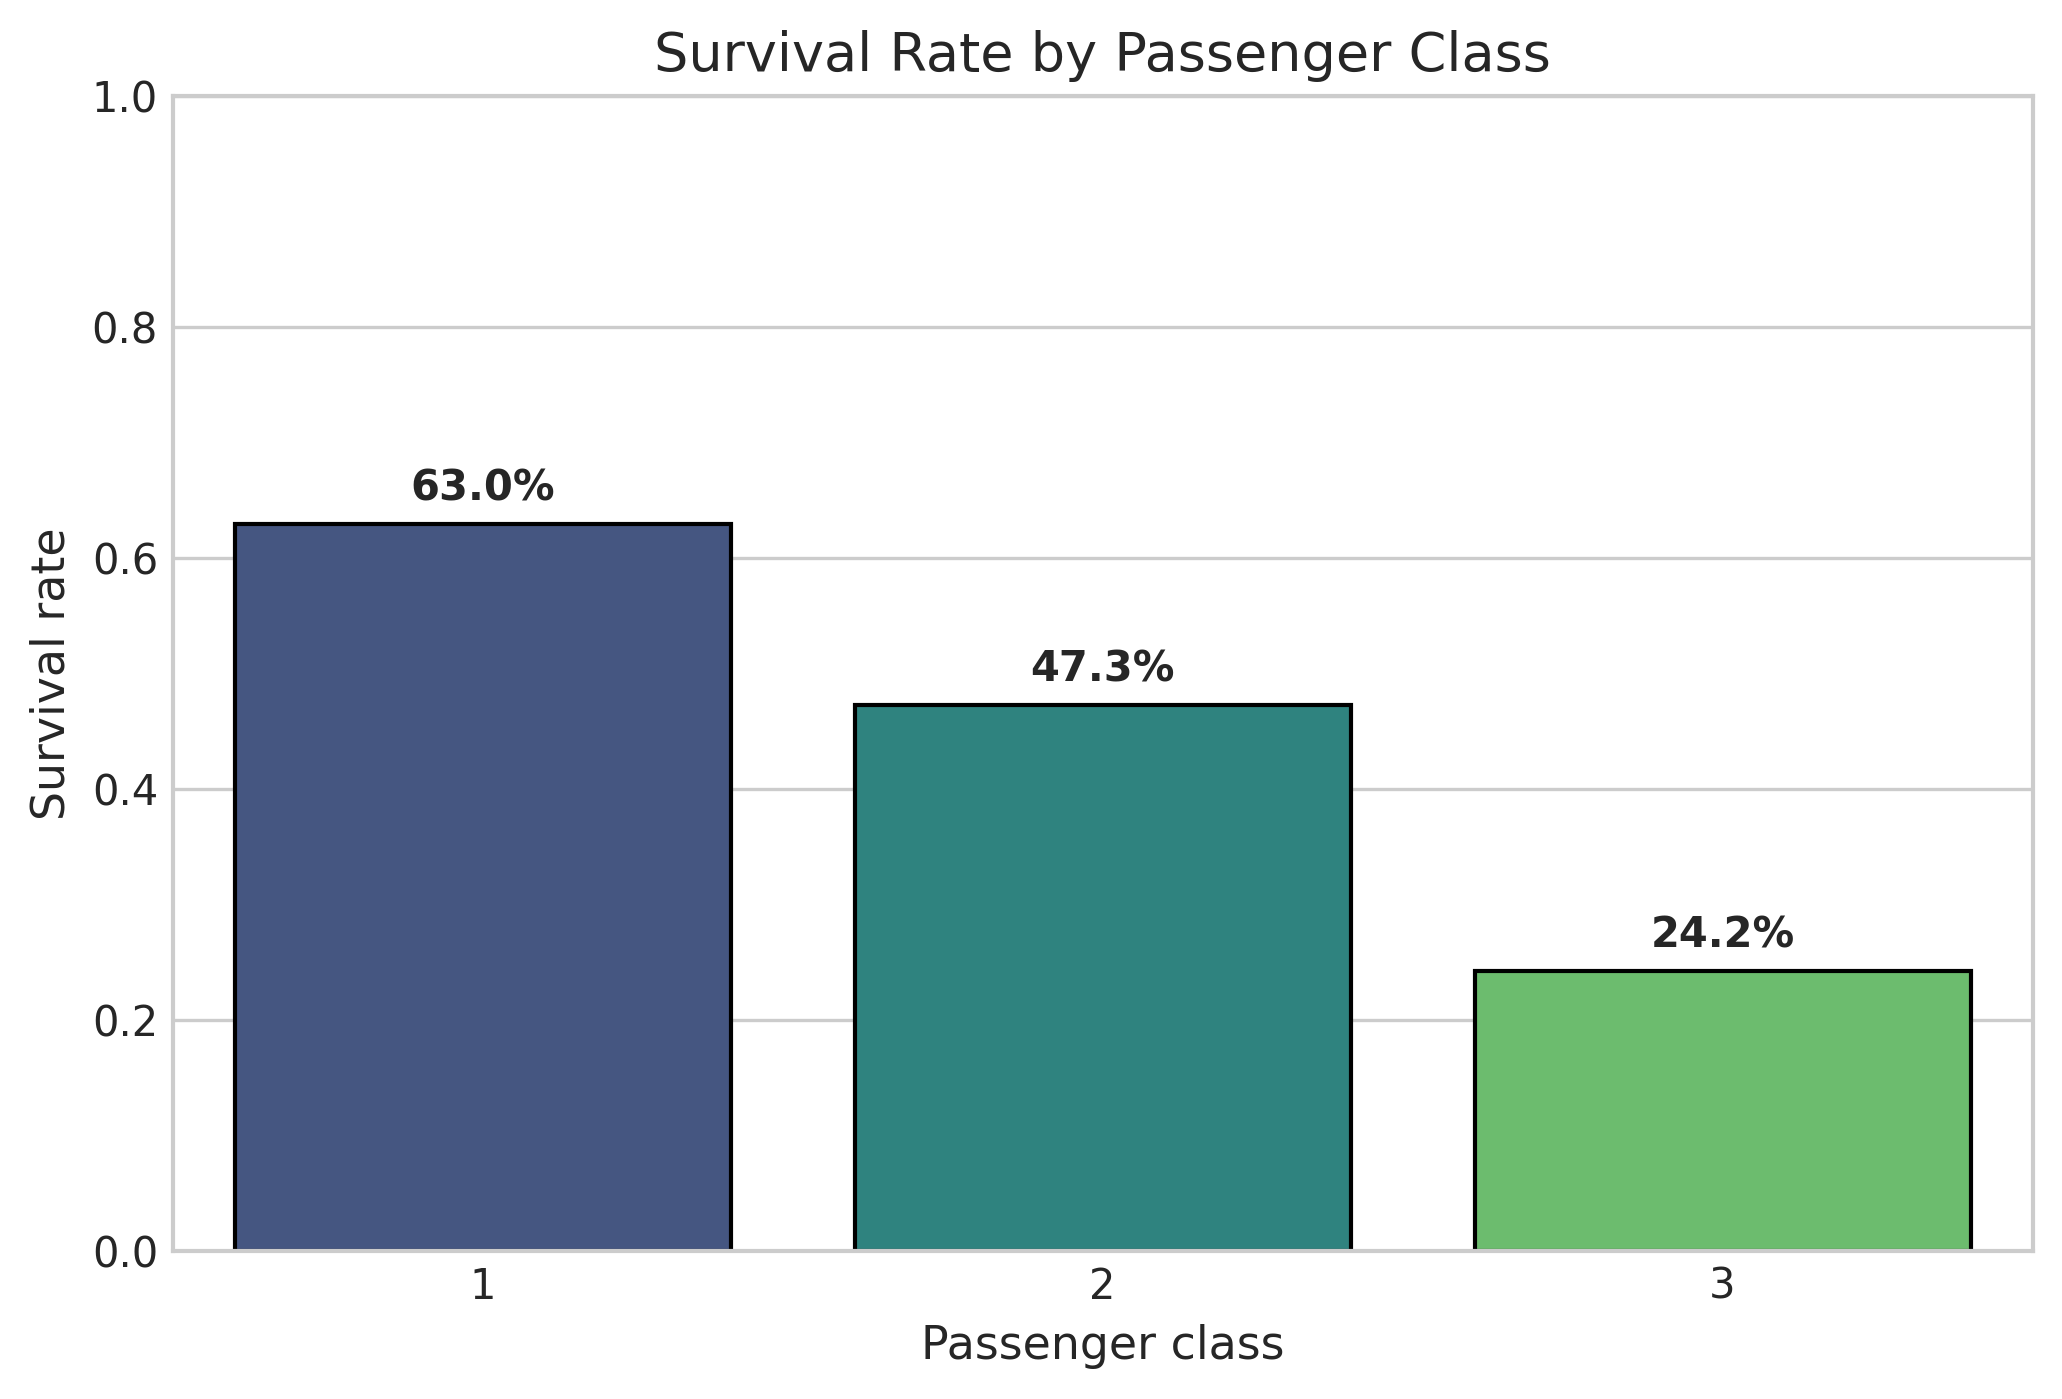
\includegraphics[width=\linewidth]{figures/survival_by_class.png}
\caption{By passenger class}
\end{subfigure}
\caption{Survival rate by the two strongest univariate predictors: female passengers
survived at $74.2\%$ versus $18.9\%$ for males; survival declines monotonically with
class.}
\label{fig:by_gender}
\end{figure}

\begin{figure}[H]
\centering
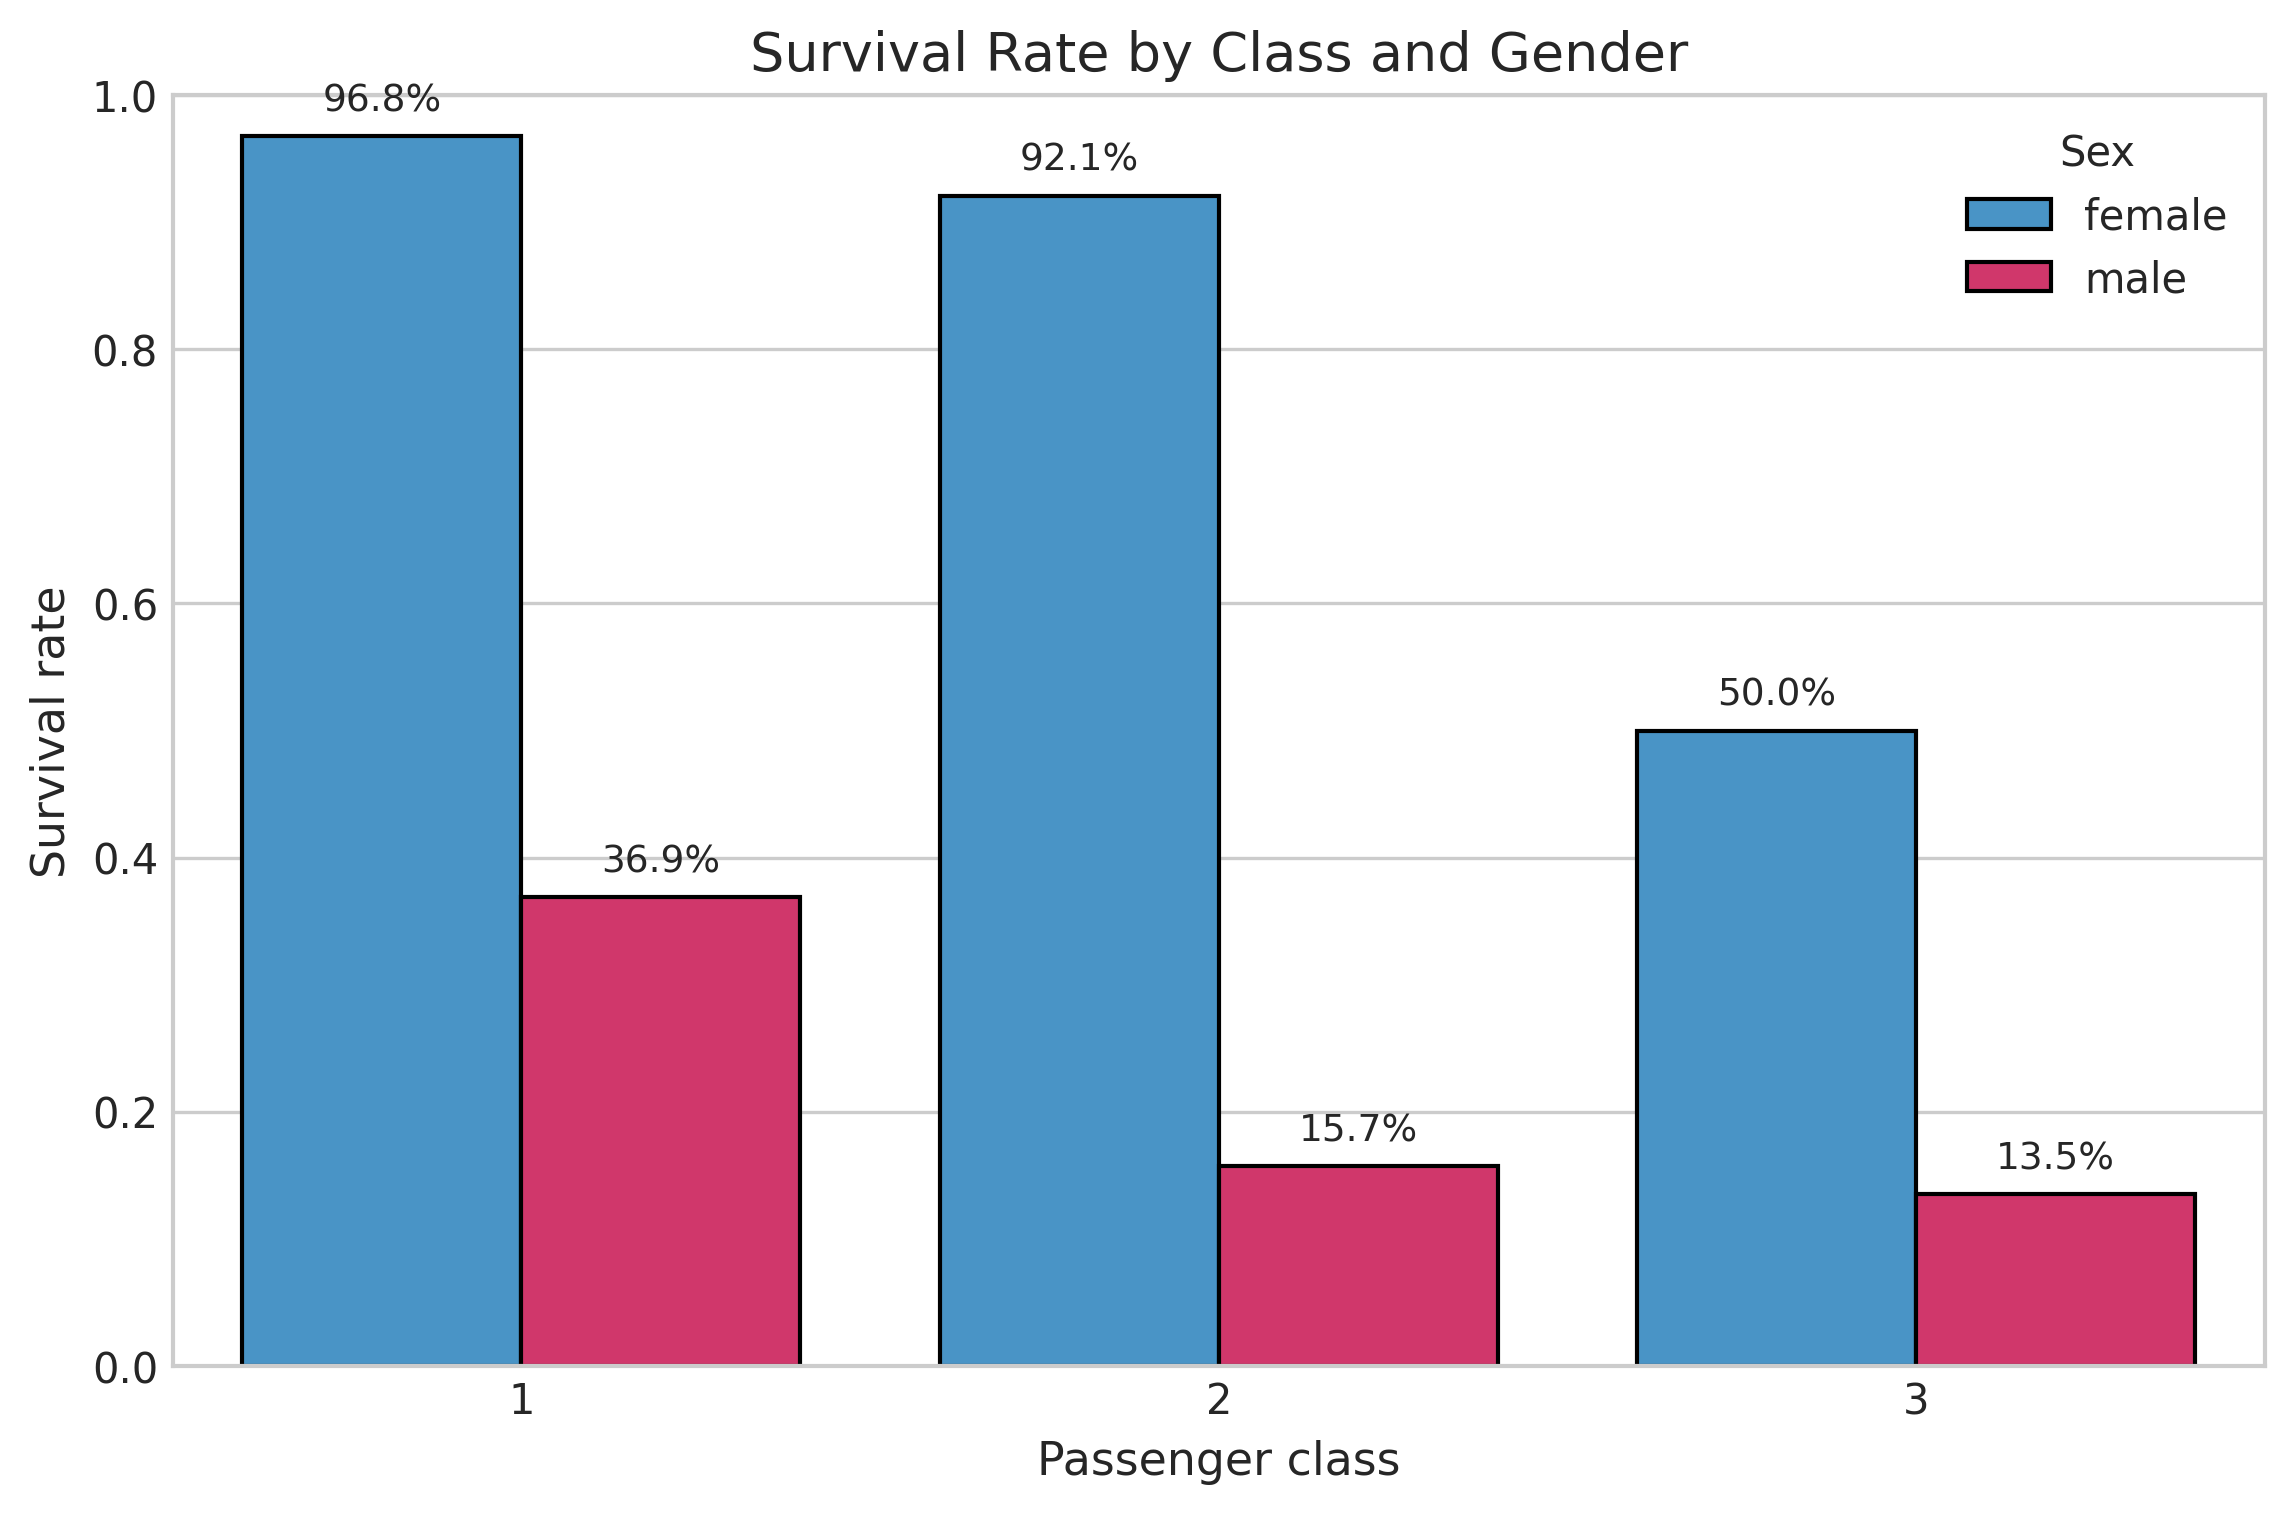
\includegraphics[width=0.98\columnwidth]{figures/survival_by_class_gender.png}
\caption{Joint effect of class and gender. First-class women survived at 96.8\% while
third-class men survived at only 13.5\%.}
\label{fig:class_gender}
\end{figure}

\begin{figure}[H]
\centering
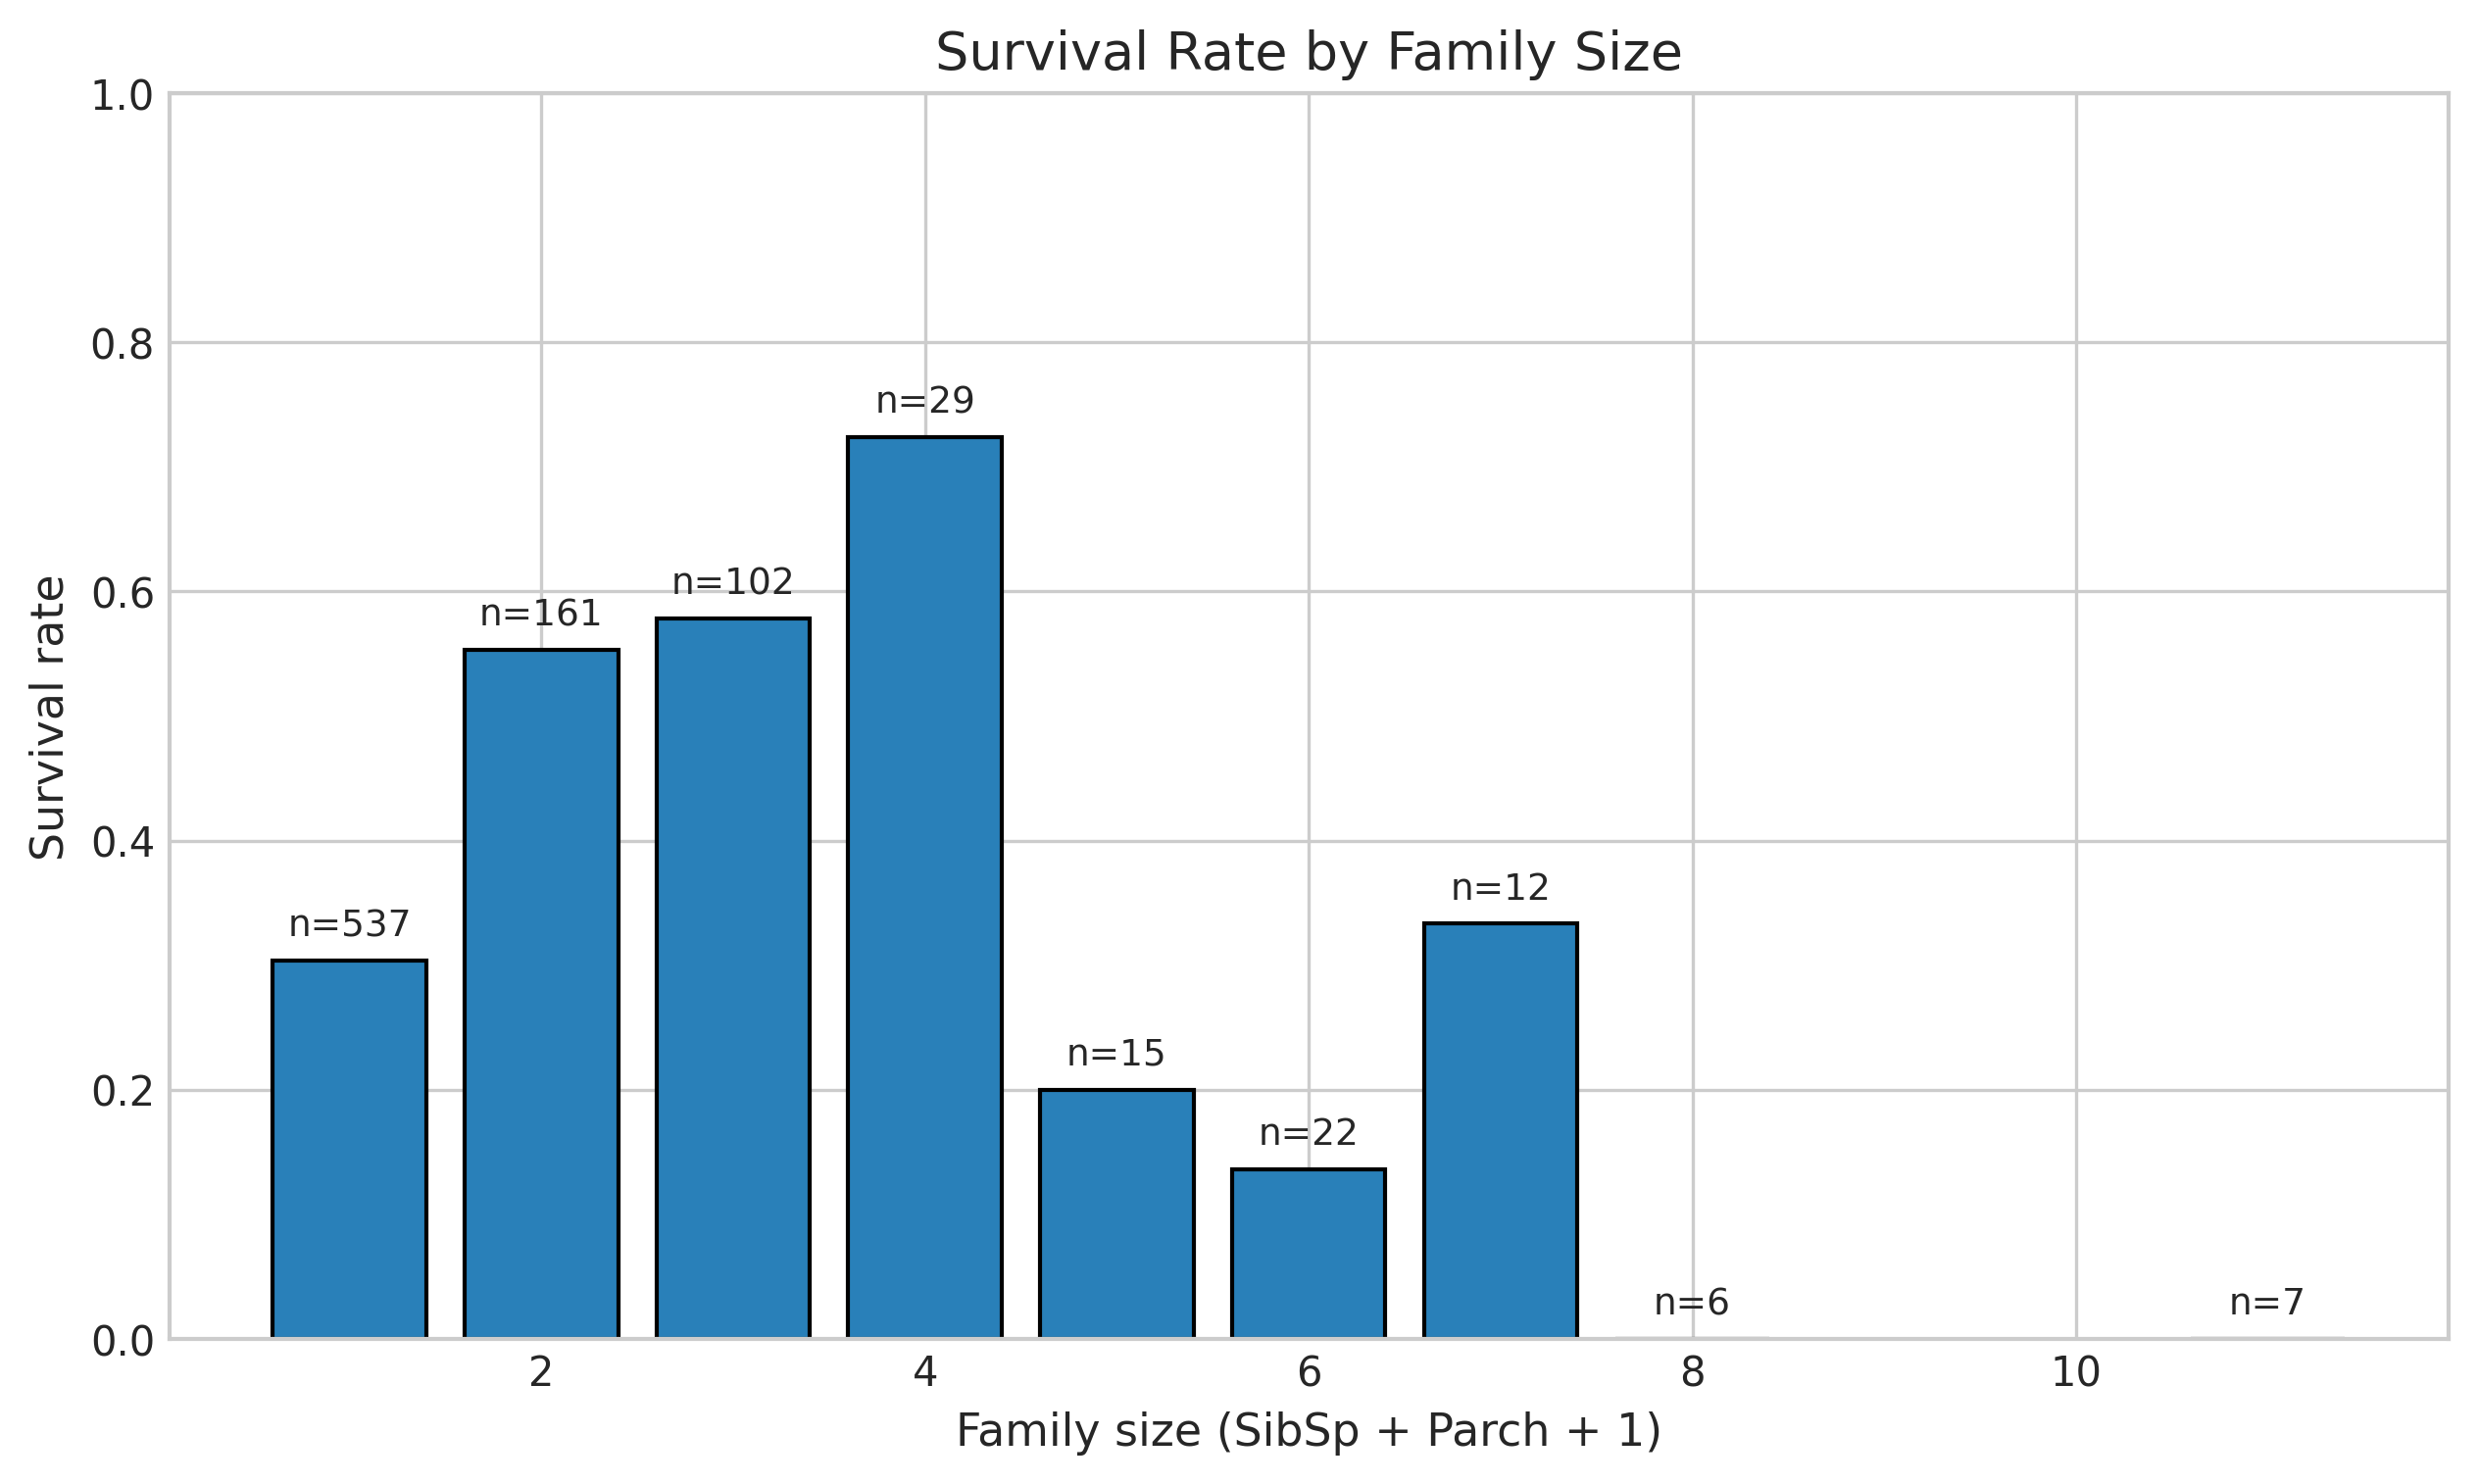
\includegraphics[width=0.95\columnwidth]{figures/family_size_survival.png}
\caption{Family-size effect. Survival peaks at family sizes of 2--4 and collapses for
very large ($\ge 5$) groups --- behaviour captured by the engineered \texttt{FamilySize}
feature.}
\label{fig:family}
\end{figure}

\begin{figure}[H]
\centering
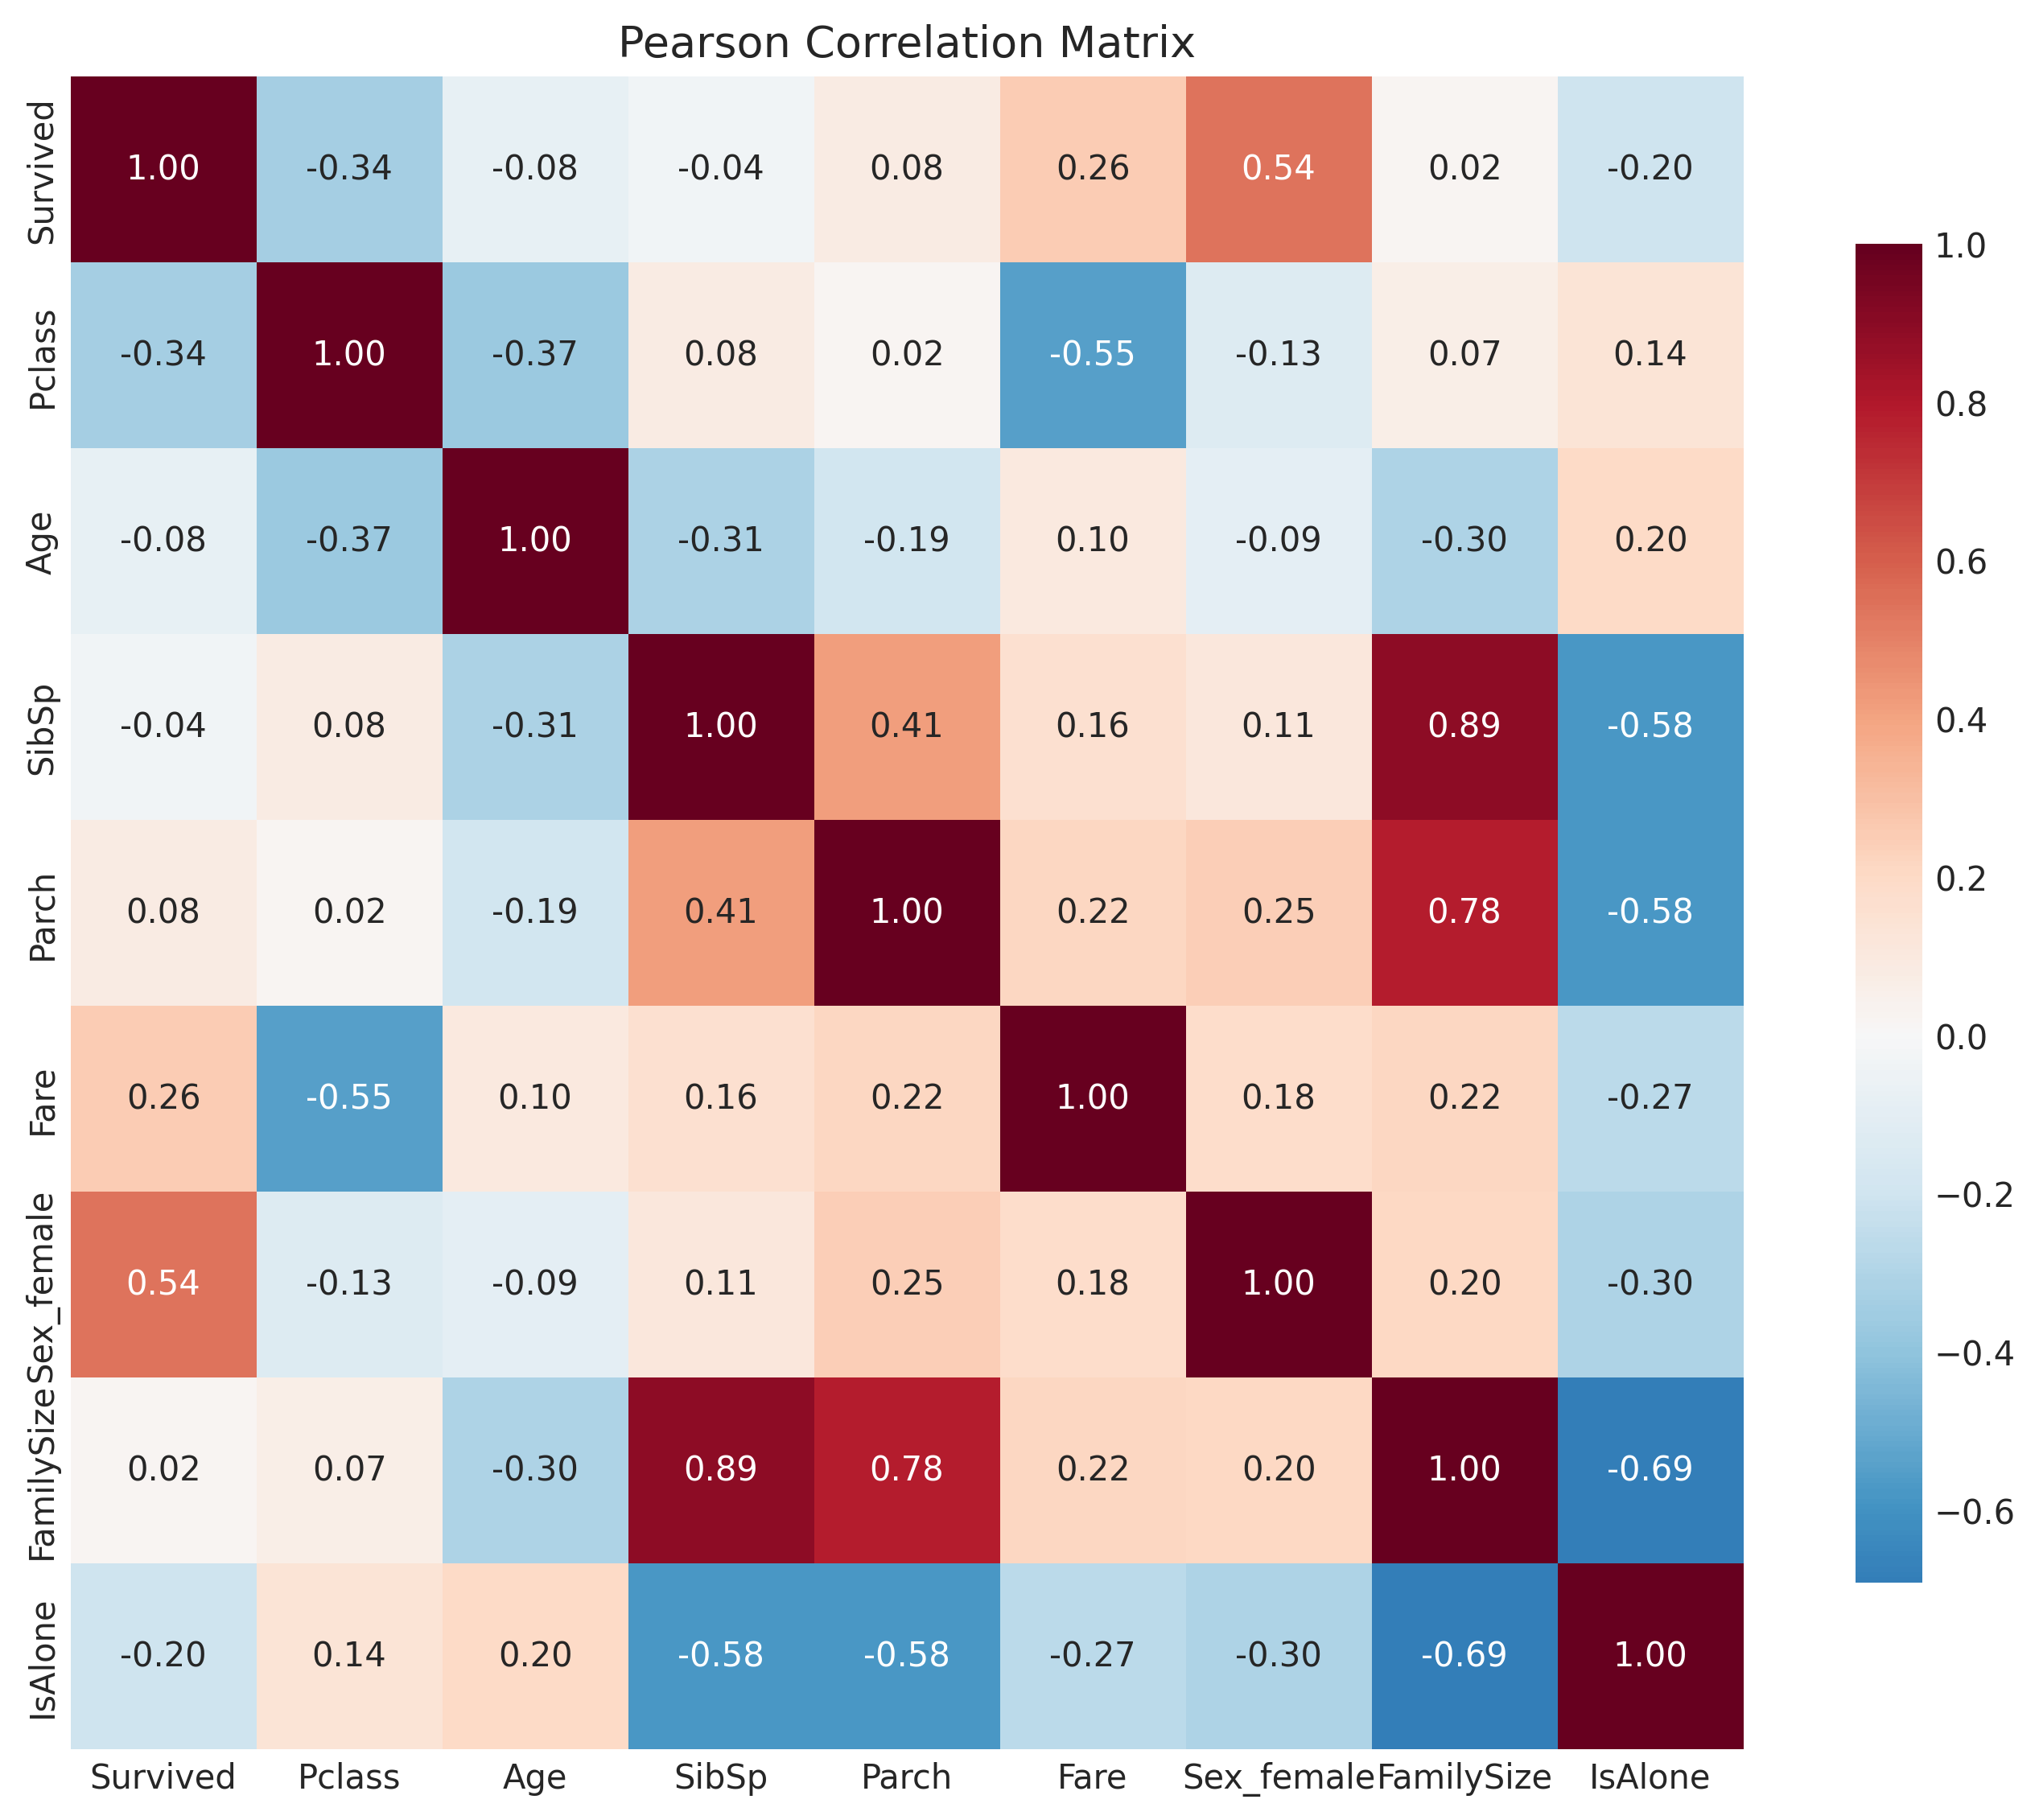
\includegraphics[width=0.98\columnwidth]{figures/correlation_heatmap.png}
\caption{Pearson correlations. The strongest predictors of \texttt{Survived} are
\texttt{Sex\_female} ($+0.54$), \texttt{Pclass} ($-0.34$), and \texttt{Fare} ($+0.26$).}
\label{fig:corr}
\end{figure}

\subsection{Model performance}
Table~\ref{tab:summary} consolidates the six primary metrics for each classifier.

\begin{table*}[t]
\centering\small
\caption{Comparative performance of four classifiers on the 179-row held-out test set
(10-fold CV on $n_\text{train}=712$).}
\label{tab:summary}
\begin{tabular}{@{}lcccccc@{}}
\toprule
Model & CV Accuracy ($\mu\pm\sigma$) & Test Accuracy & Precision & Recall & F1 & AUC \\
\midrule
Na\"ive Bayes          & $0.6572 \pm 0.1169$ & $0.6257$ & $0.5083$ & $0.8841$ & $0.6455$ & $0.7782$ \\
Decision Tree          & $0.8202 \pm 0.0363$ & $0.8156$ & $0.7903$ & $0.7101$ & $0.7481$ & $0.8375$ \\
Logistic Regression    & $0.8146 \pm 0.0393$ & $\mathbf{0.8324}$ & $0.8000$ & $0.7536$ & $\mathbf{0.7761}$ & $\mathbf{0.8644}$ \\
Random Forest          & $0.8131 \pm 0.0336$ & $0.8101$ & $0.7778$ & $0.7101$ & $0.7424$ & $0.8286$ \\
\bottomrule
\end{tabular}
\end{table*}

\begin{figure}[H]
\centering
\begin{subfigure}{0.49\columnwidth}
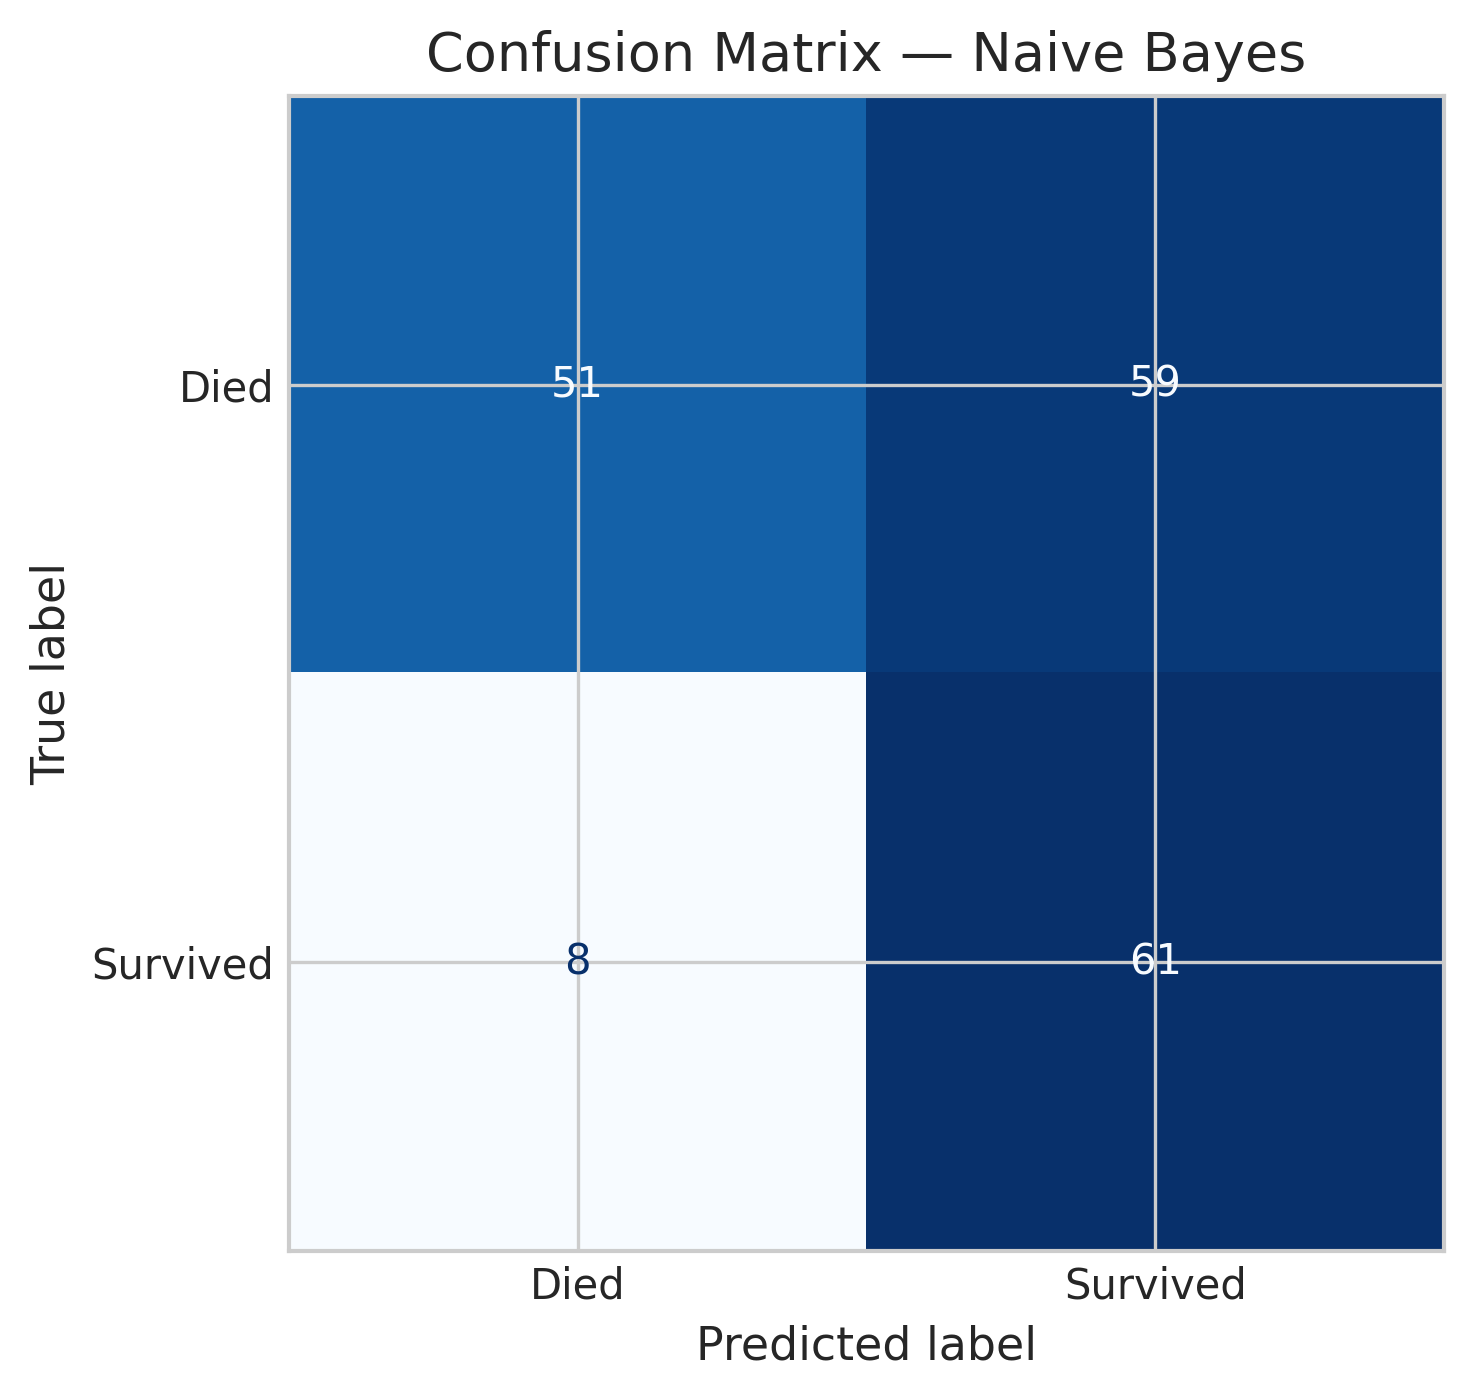
\includegraphics[width=\linewidth]{figures/confusion_matrix_nb.png}
\caption{Na\"ive Bayes}
\end{subfigure}\hfill
\begin{subfigure}{0.49\columnwidth}
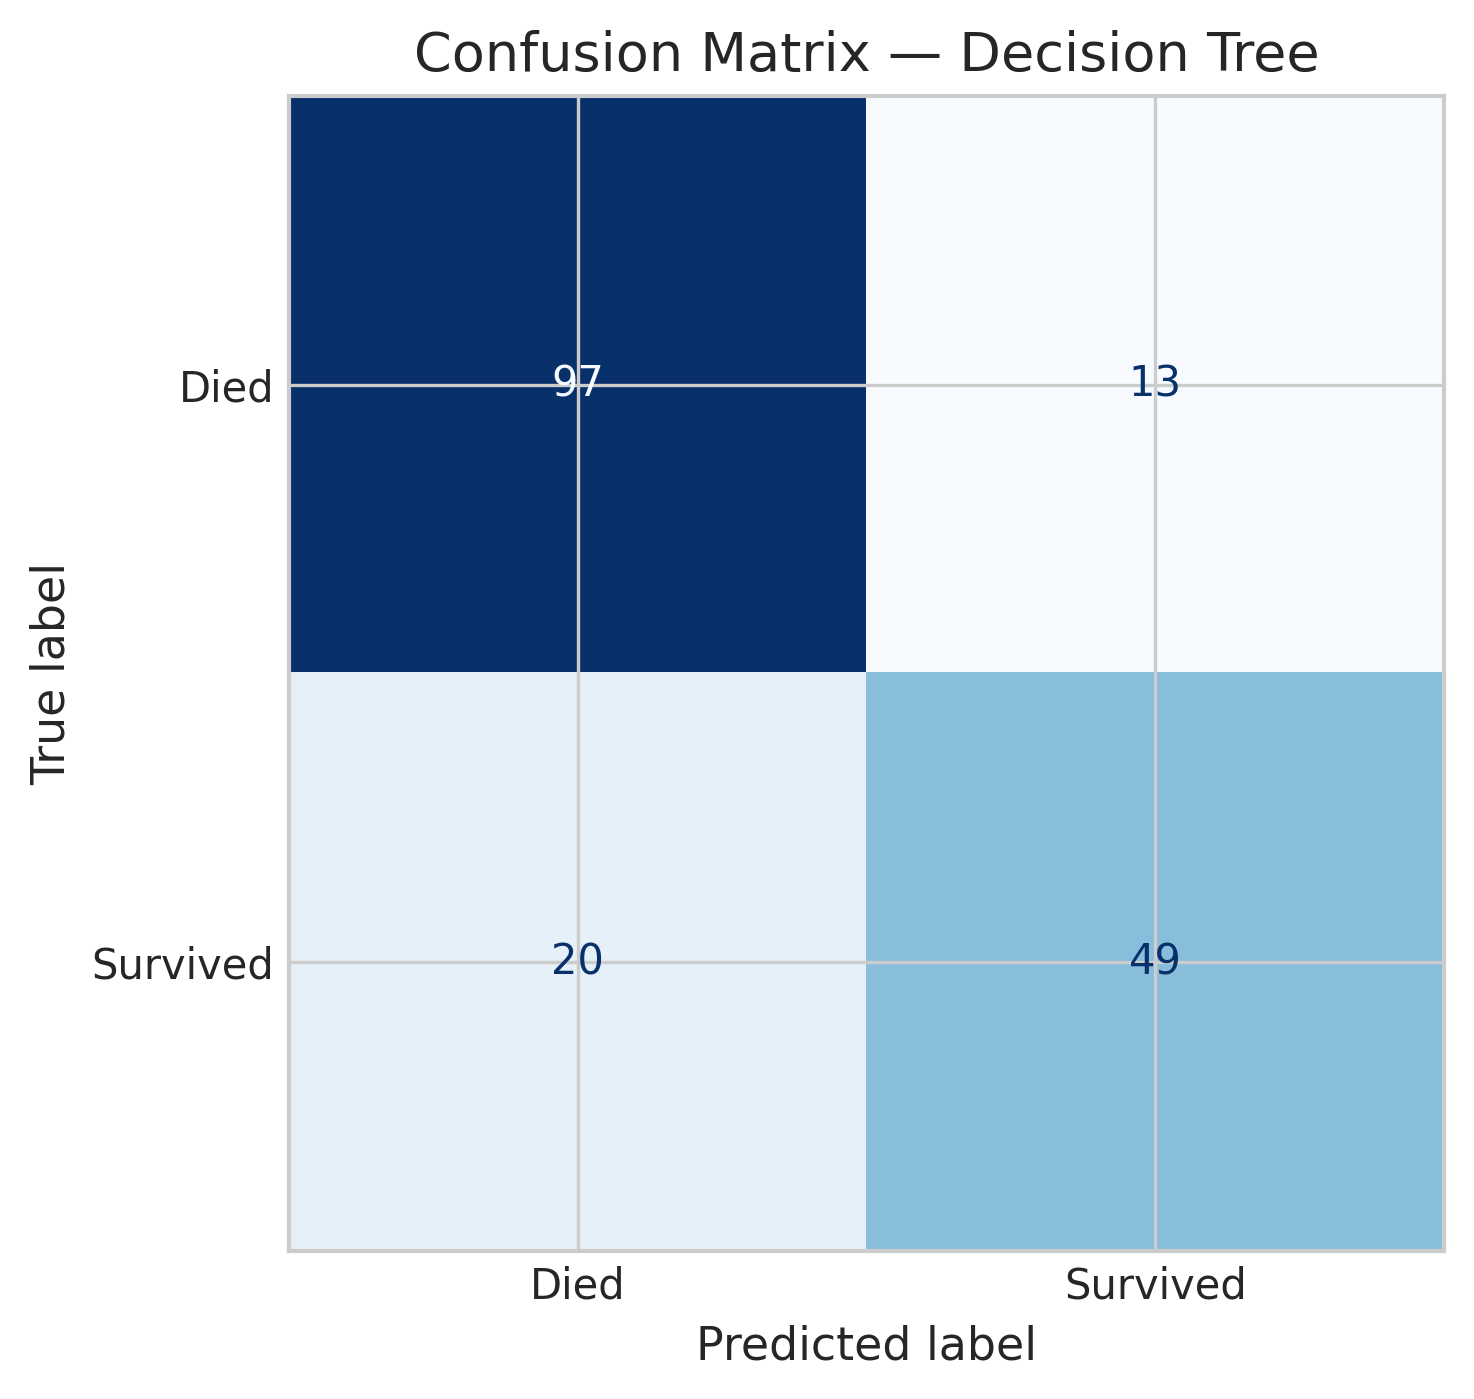
\includegraphics[width=\linewidth]{figures/confusion_matrix_dt.png}
\caption{Decision Tree}
\end{subfigure}
\caption{Confusion matrices on the held-out test set. Na\"ive Bayes over-predicts the
positive class (59 false positives), whereas the Decision Tree is materially better
balanced.}
\label{fig:cm}
\end{figure}

\begin{figure}[H]
\centering
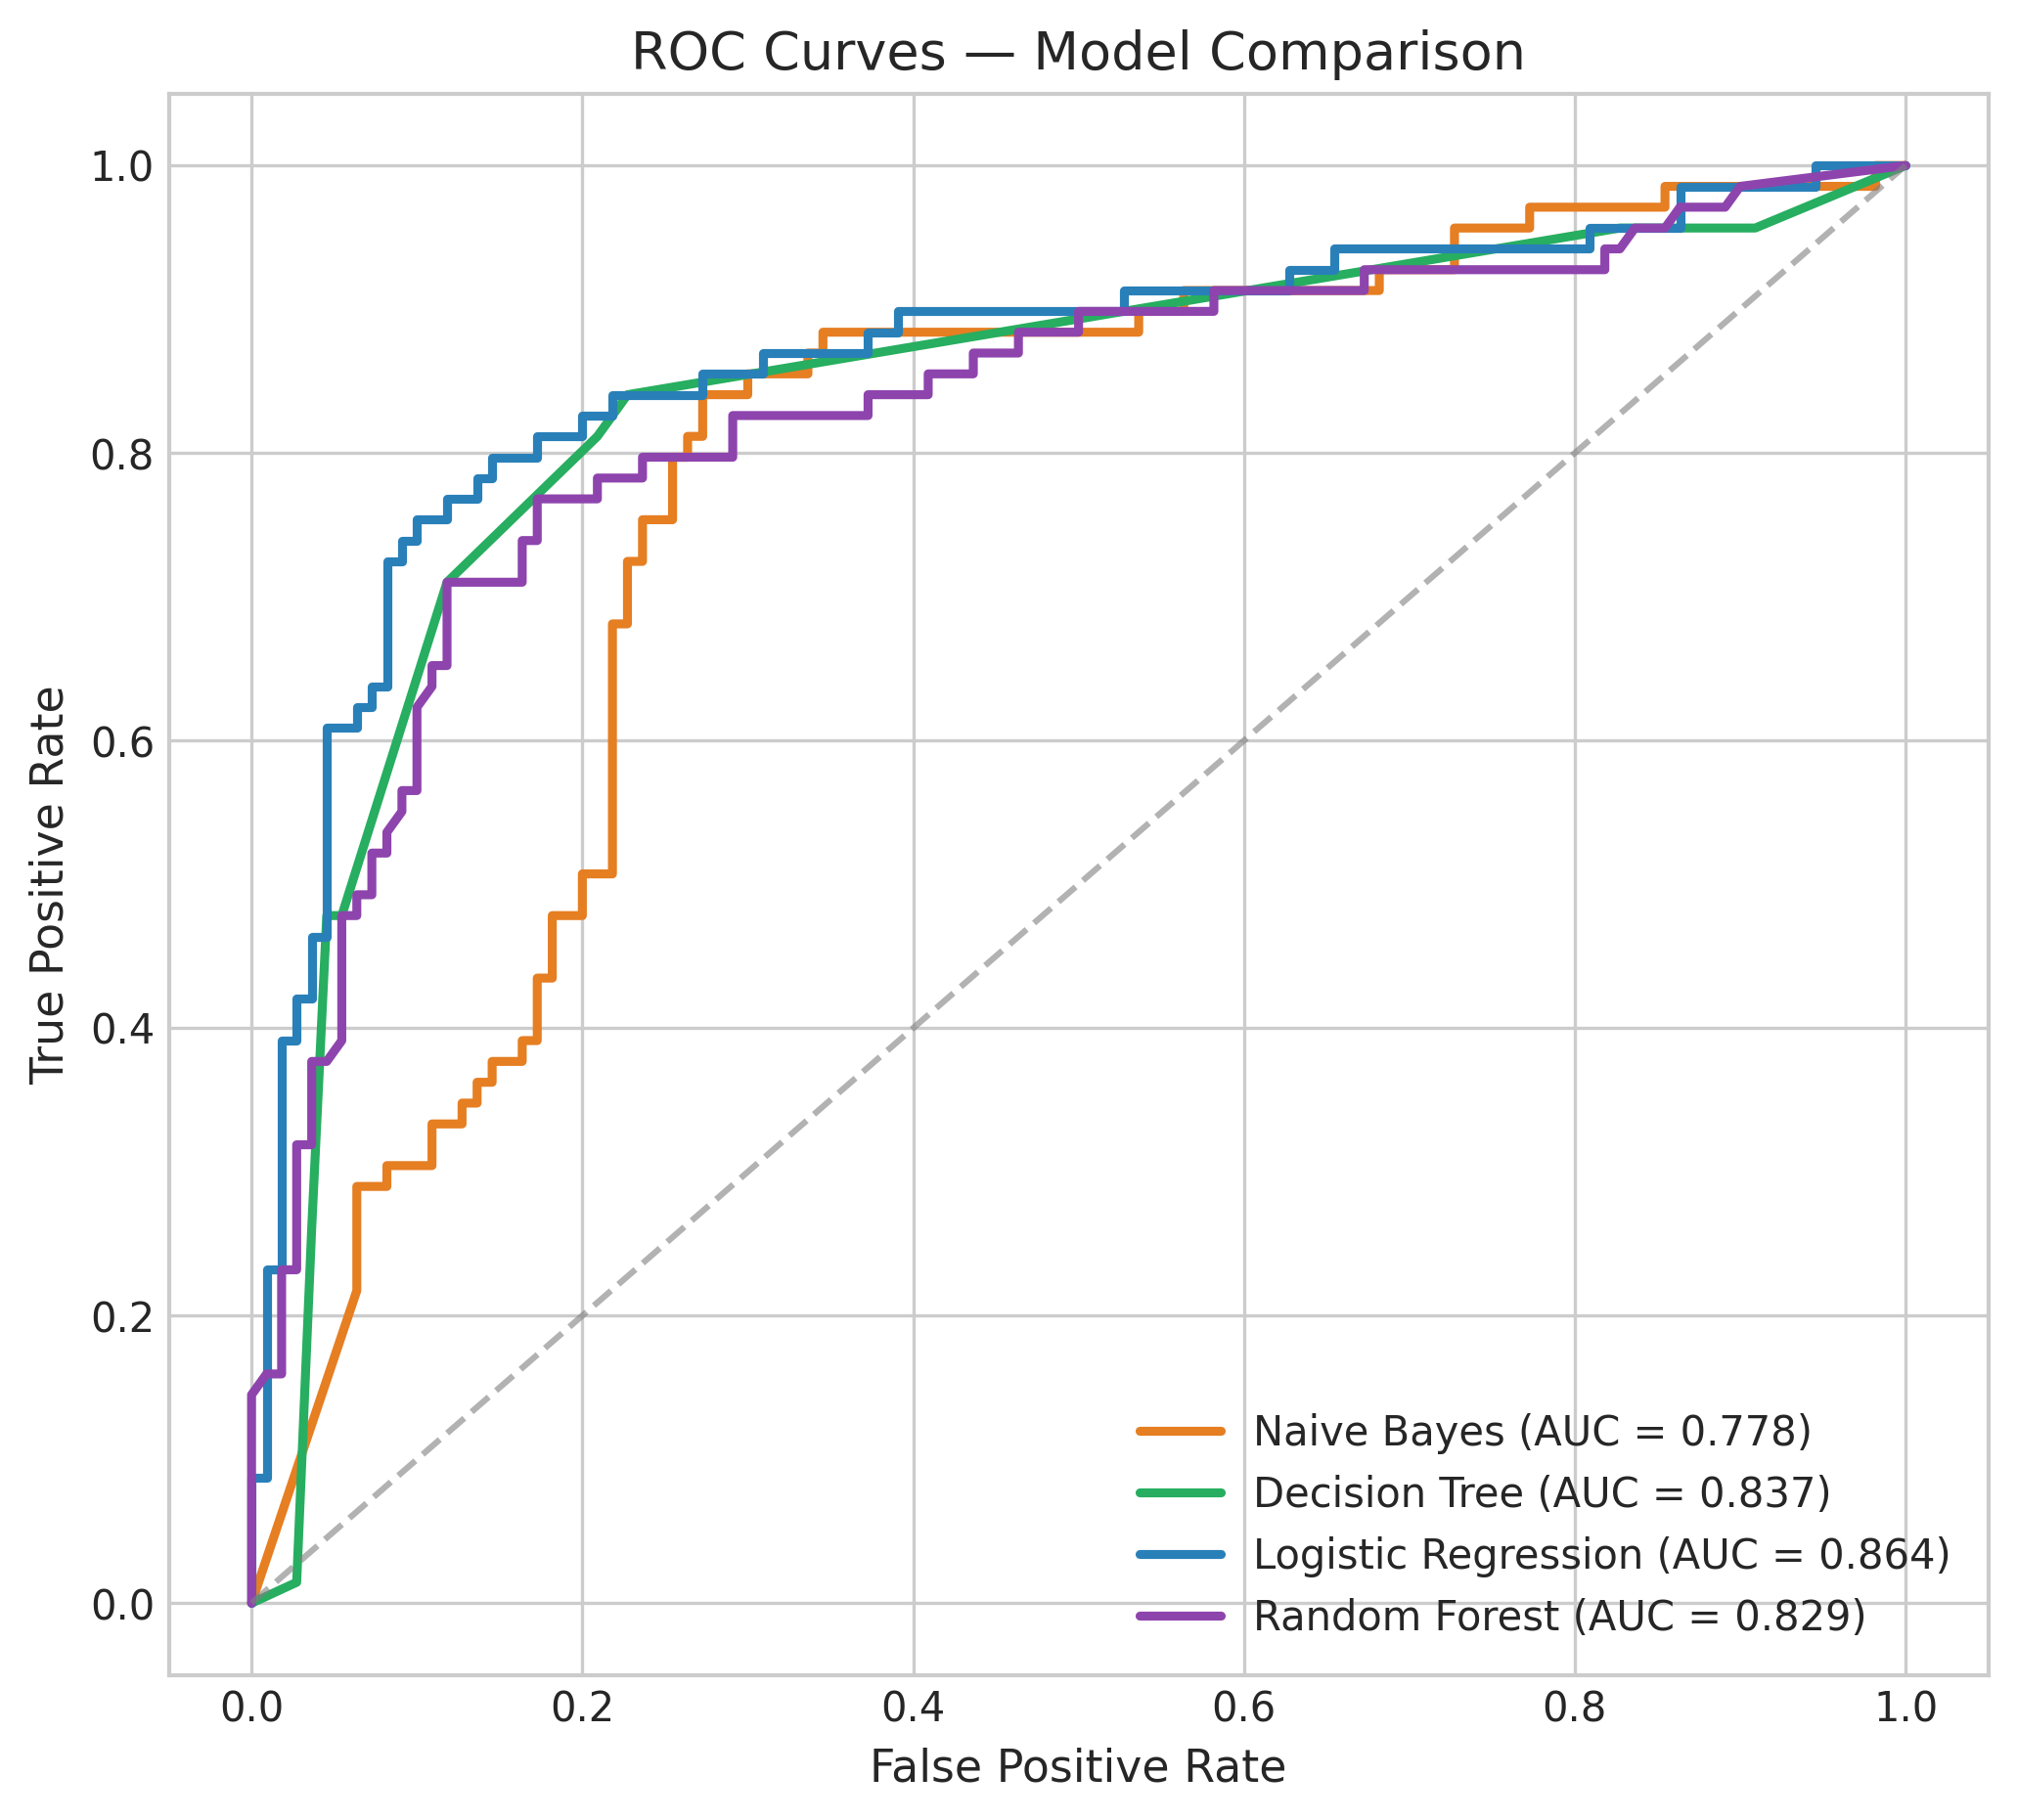
\includegraphics[width=0.98\columnwidth]{figures/roc_curves.png}
\caption{ROC curves for all four classifiers. Logistic Regression dominates slightly
across most thresholds (AUC $= 0.864$); Na\"ive Bayes trails uniformly.}
\label{fig:roc}
\end{figure}

\begin{figure}[H]
\centering
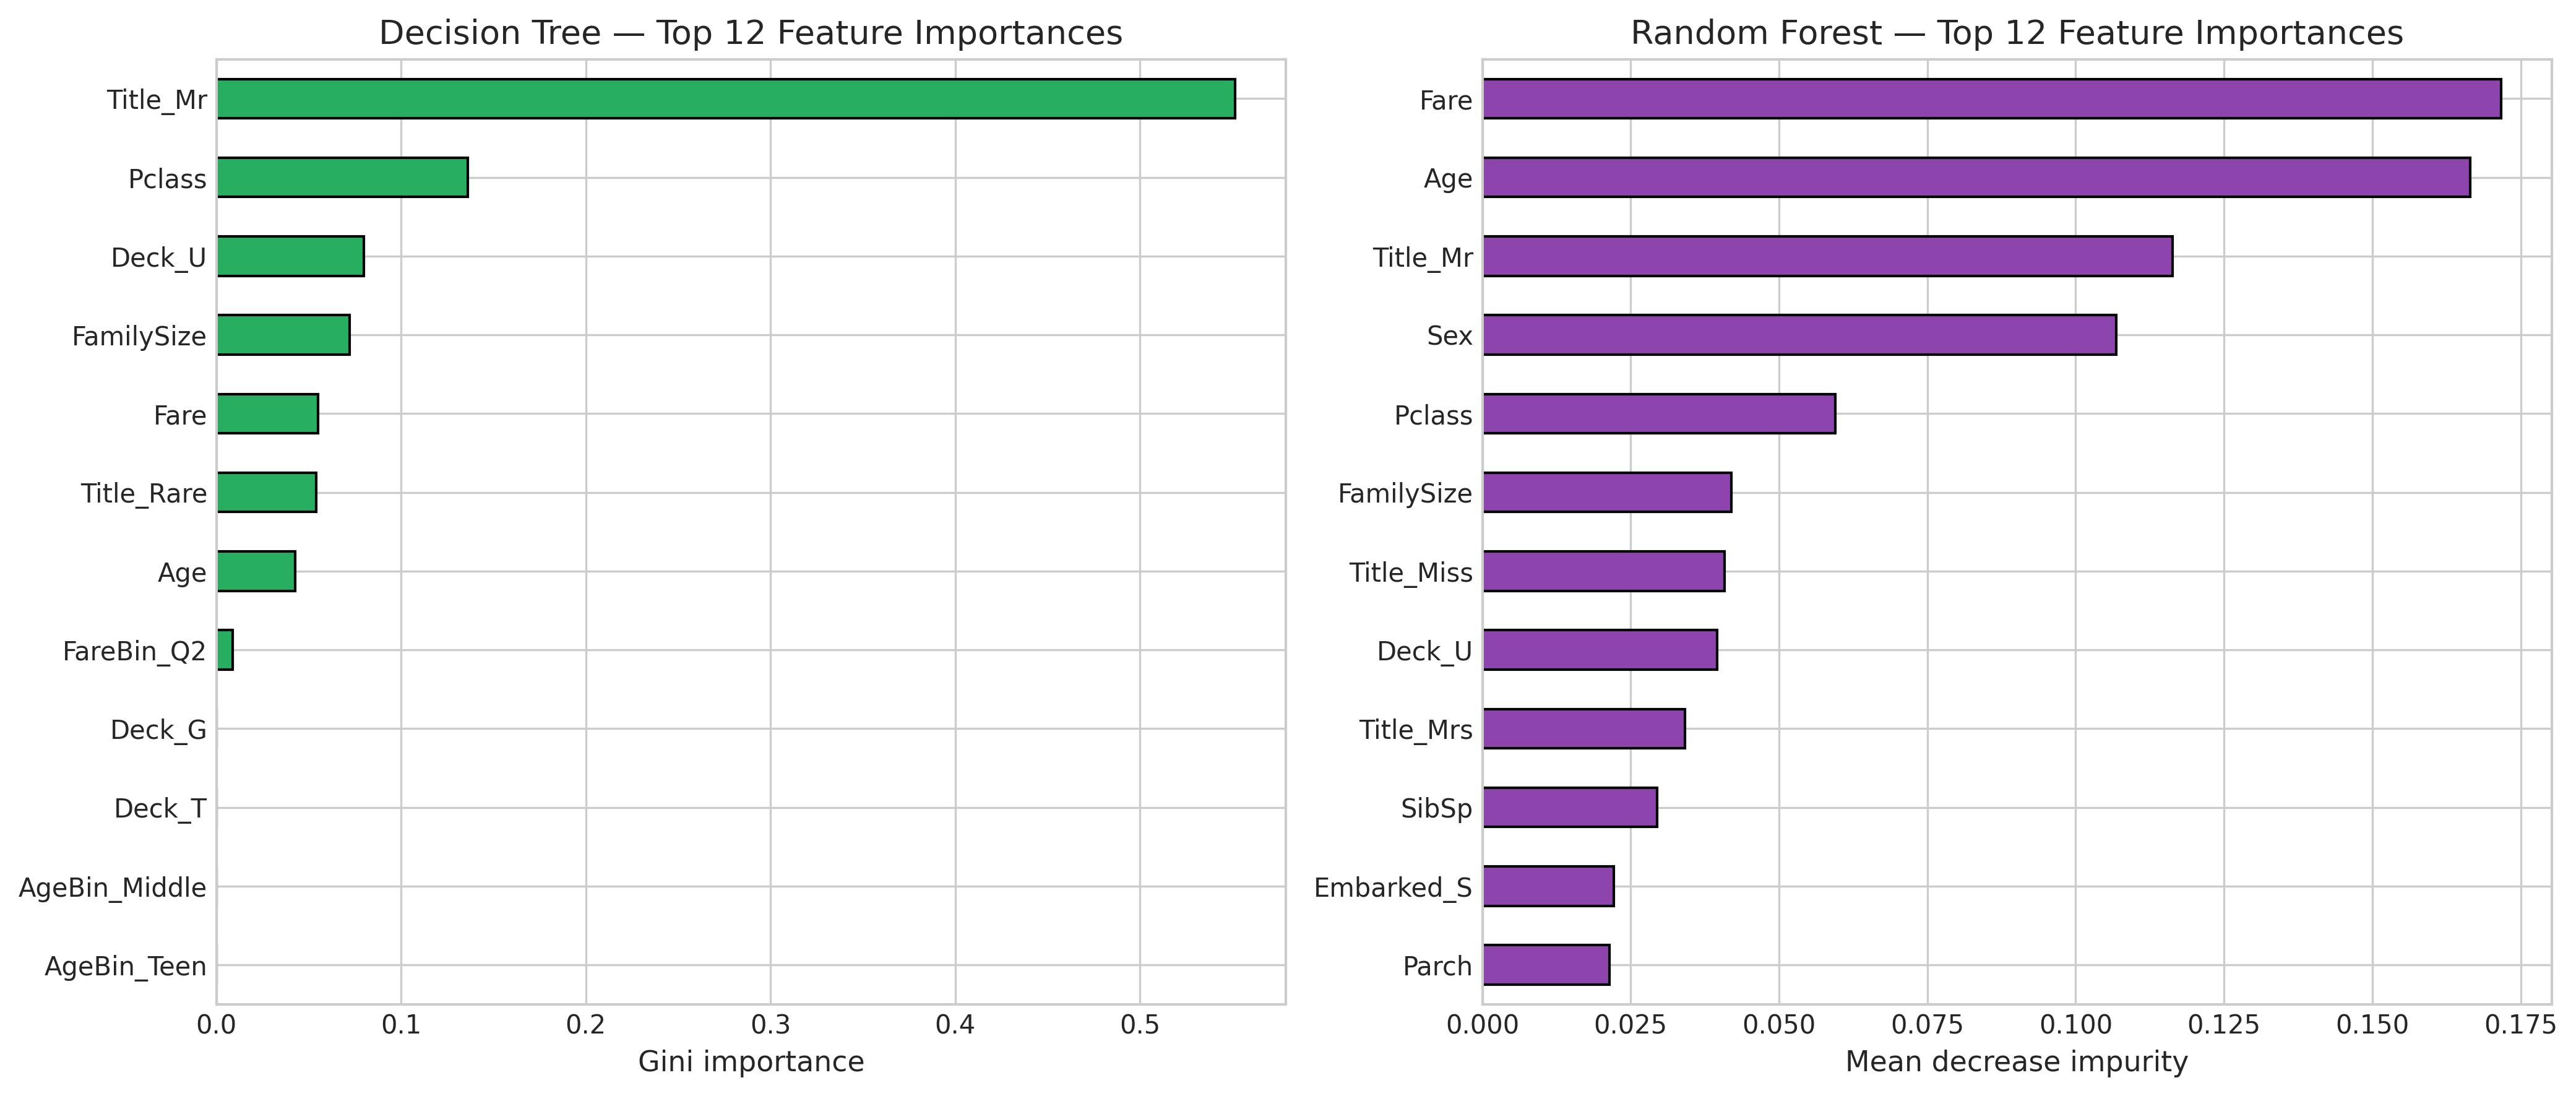
\includegraphics[width=0.98\columnwidth]{figures/feature_importance.png}
\caption{Top-12 feature importances. The Decision Tree concentrates split weight on
\texttt{Title\_Mr} and \texttt{Pclass}; the Random Forest distributes importance more
evenly across \texttt{Fare}, \texttt{Age}, and \texttt{Title\_Mr}.}
\label{fig:feat}
\end{figure}

\begin{figure*}[t]
\centering
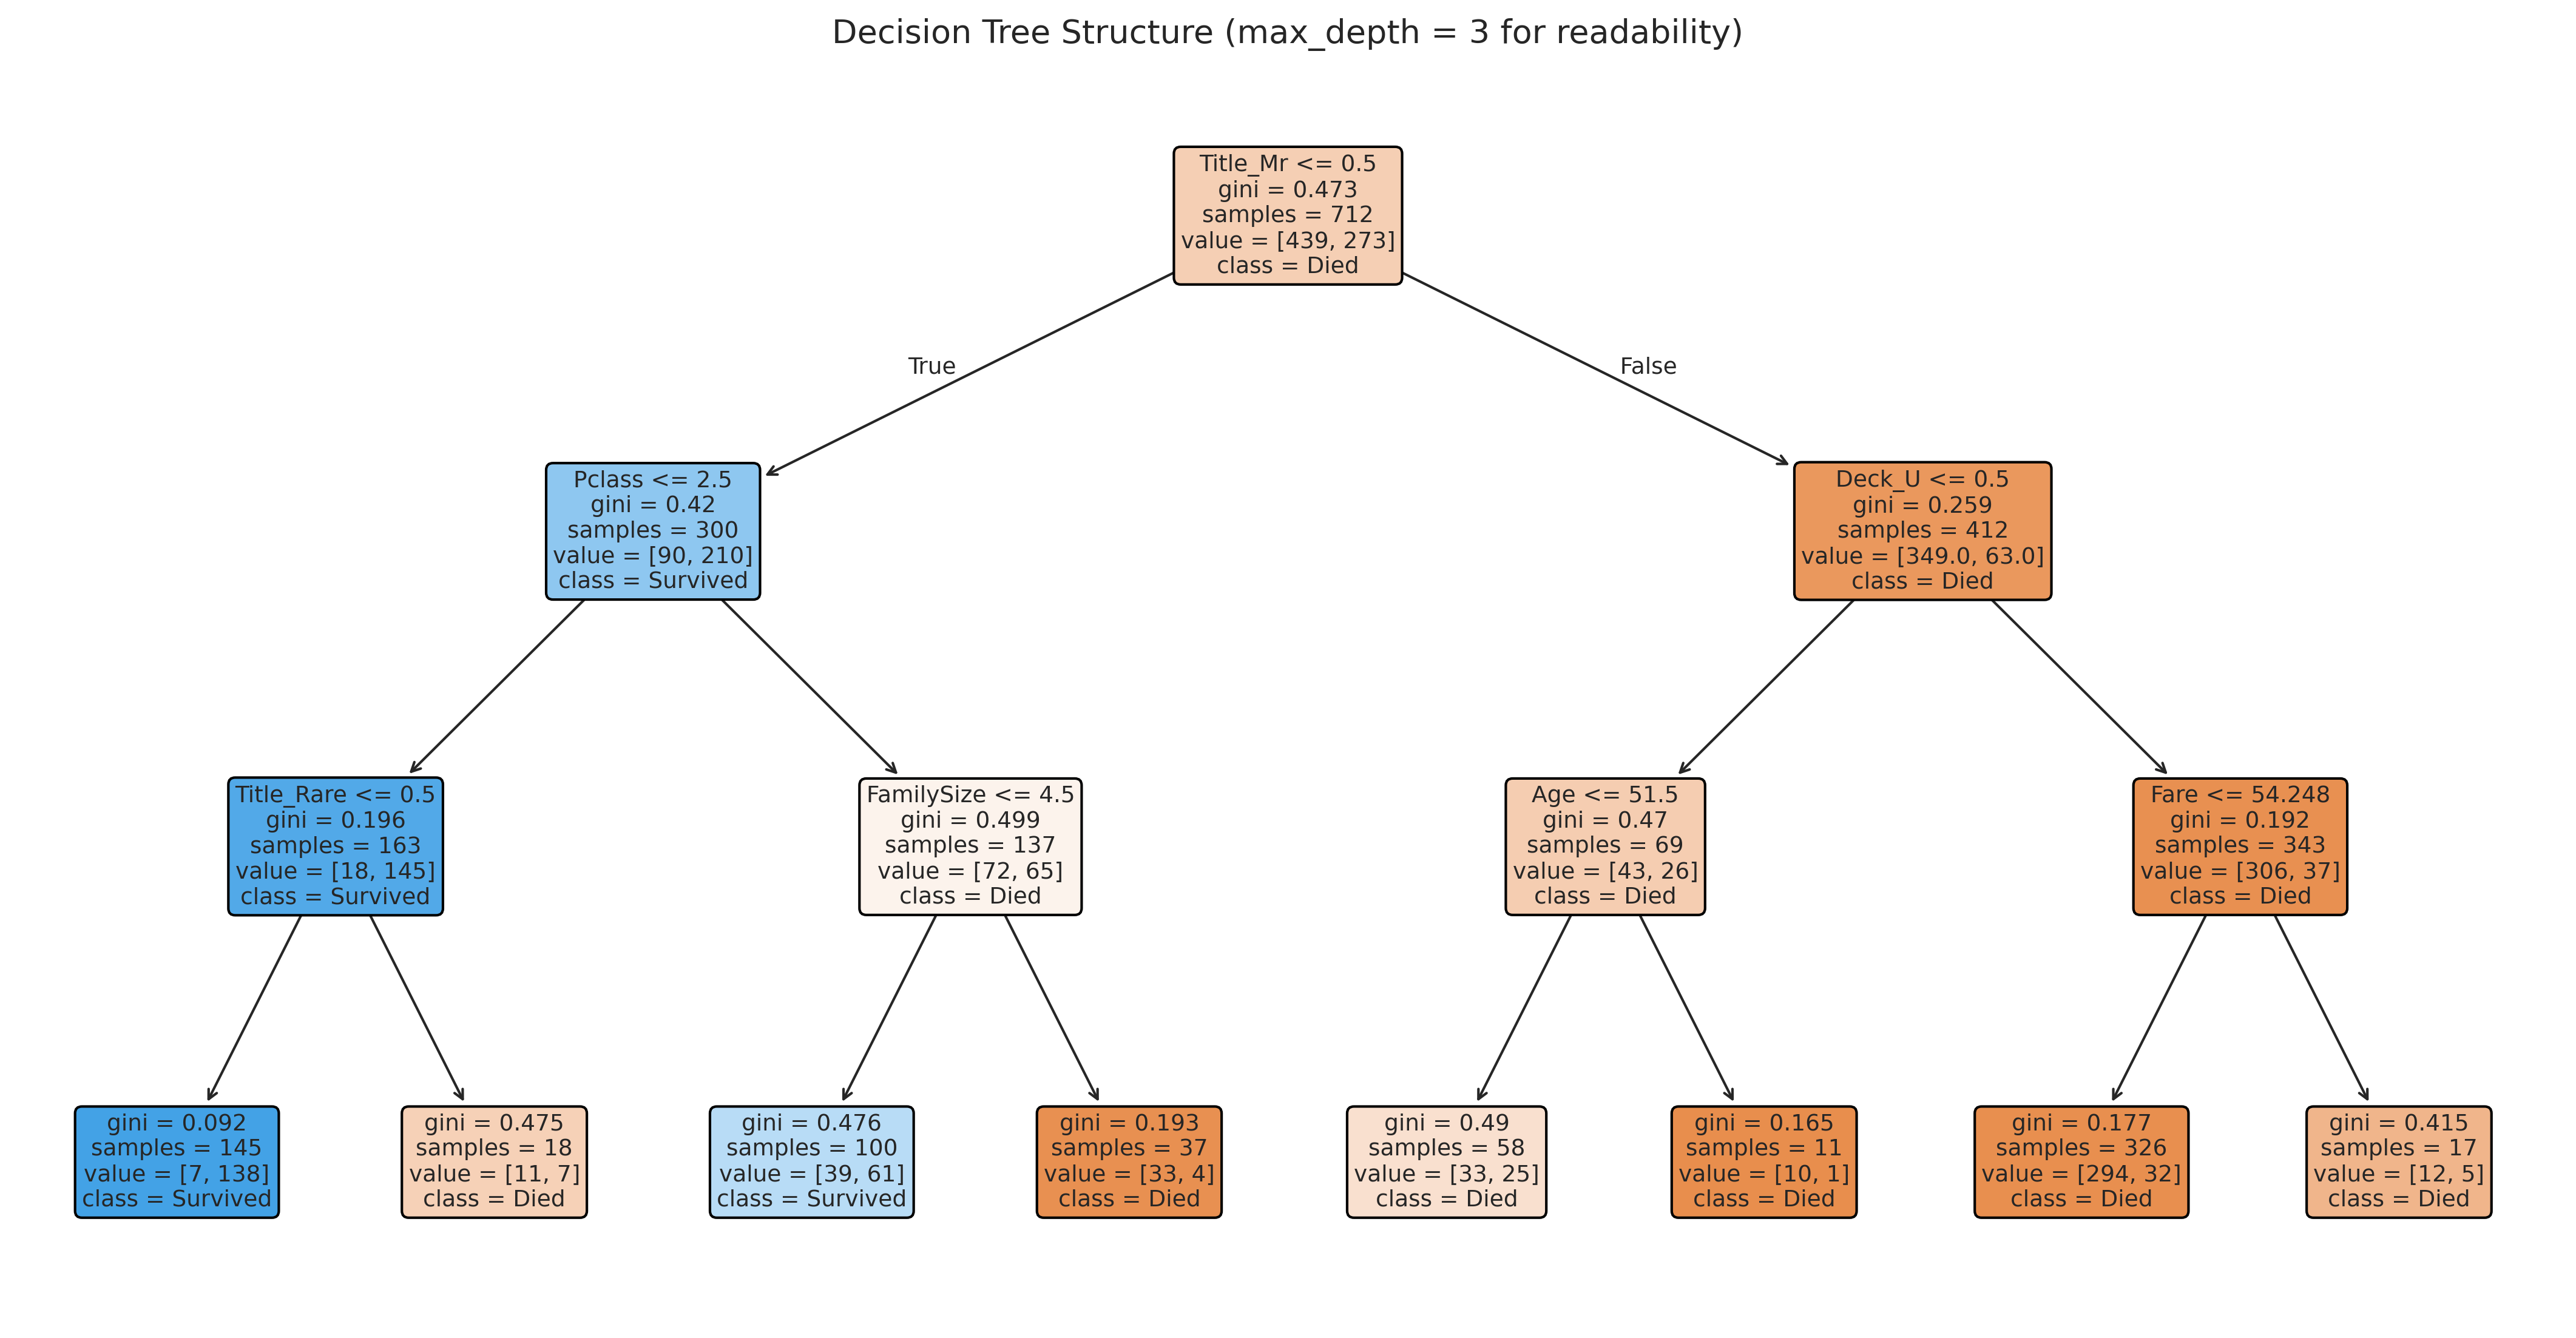
\includegraphics[width=0.92\textwidth]{figures/decision_tree_viz.png}
\caption{Fitted Decision Tree (\texttt{max\_depth}=3 shown for readability; the
deployed model uses depth 4). The root split on \texttt{Title\_Mr} captures the bulk
of the gender / honorific signal in a single question.}
\label{fig:tree}
\end{figure*}

\subsection{Statistical significance: NB vs.\ DT}
On the $n_\text{test}=179$ paired predictions the disagreement counts are $b=12$
(NB correct, DT wrong) and $c=46$ (NB wrong, DT correct). The exact McNemar test yields
\[
p \;=\; 8.22\times 10^{-6} ,
\]
so the null hypothesis of equal error rates is rejected at any conventional level.
The $\approx 19$ percentage-point gap between NB and DT is not a sampling artefact.

\subsection{Discussion}
Three findings stand out.

\paragraph{NB underperforms because its assumptions fail here.} The one-hot expansion of
categorical features (Title, Deck, AgeBin, FareBin) introduces many strongly
correlated dummy variables, directly violating
Equation~\eqref{eq:nb_independence}. Modelling binary dummies as Gaussians
compounds the mismatch. This is the textbook failure mode of Gaussian NB on
engineered tabular data and is the principal cause of its low AUC.

\paragraph{Gender dominates, class modulates.} Both the Decision Tree (Fig.~\ref{fig:feat}
left) and the Random Forest (Fig.~\ref{fig:feat} right) place \texttt{Title\_Mr},
\texttt{Pclass}, and \texttt{Fare} in the top four. The root split of the learned tree
(Fig.~\ref{fig:tree}) is a single test on \texttt{Title\_Mr}, which perfectly isolates
adult males whose survival rate is $<20\%$. This is precisely the ``women and children
first'' protocol recovered from the data.

\paragraph{Linear structure is nearly sufficient.} Logistic Regression attains the highest
test accuracy (83.24\%) and AUC (0.864), indicating that after feature engineering the
decision boundary is close to linear. Random Forest does not outperform the single
Decision Tree, which suggests that the feature set encodes the important interactions
explicitly (\texttt{FamilySize}, \texttt{IsAlone}, \texttt{Title}) rather than requiring
tree bagging to discover them.

\paragraph{Limitations.} (i) The study uses a single fixed hold-out fold; repeated
nested CV would tighten the accuracy intervals. (ii) We compare Gaussian NB against
alternatives; a categorical- or multinomial-NB that respects the type of our
one-hot dummies would be a fairer probabilistic comparator. (iii) No hyper-parameter
search is performed for Logistic Regression or Random Forest beyond defaults.

% =============================================================================
\section{Implications and Applications}\label{sec:implications}
% =============================================================================

\paragraph{Risk and insurance.} The Bayesian framing of Eq.~\eqref{eq:bayes} is the
conceptual ancestor of actuarial risk pricing: class priors and feature-conditional
likelihoods are updated into individualised posteriors. The Decision Tree, by contrast,
maps onto rule-based underwriting in which an applicant is classified through a short
sequence of questions --- a structure still used in modern claims-triage systems.

\paragraph{Emergency response and crisis planning.} The feature rankings surface
non-demographic drivers (family size, deck, fare band) that real evacuation doctrine
has to reckon with. A fielded planner should not rely purely on demographic tags but
should include mobility-proxy features of the sort we engineer here.

\paragraph{Algorithmic fairness and auditing.} The same dataset is an instructive target
for bias auditing: the strongest predictor of survival is a protected attribute, so any
deployed classifier would learn and reproduce historical inequalities. The comparison
between NB (probabilistic, harder to audit feature-by-feature) and DT (rule-based,
auditable) is directly relevant to regulatory transparency frameworks.

\paragraph{Pedagogical value.} The pipeline demonstrates every stage of the KDD process in
a single coherent exercise, at a problem size that remains tractable on a laptop --- a
property we exploit to ensure every student can reproduce the exact numbers reported
here by re-running the companion Jupyter notebook.

% =============================================================================
\section{Individual Contributions}\label{sec:contrib}
% =============================================================================
\begin{table}[H]
\centering\small
\caption{Division of work within the five-member team.}
\label{tab:contrib}
\begin{tabular}{@{}p{0.28\columnwidth}p{0.62\columnwidth}@{}}
\toprule
Member & Contributions \\
\midrule
Sarin Vadakke Thayyil & Project management and lead data architecture. Defined the 80/20
stratified evaluation protocol, authored the Methodology and Implications sections, and
coordinated all deliverables. \\
\addlinespace
Lekshmi S~S & Principal research and algorithm specialisation. Comparative analysis of
Gini vs.\ entropy splits; drafted the Literature Review. \\
\addlinespace
Akbar T E & Visualisation engineering and data storytelling. Produced every figure in
this manuscript and maintained the consistent visual language. \\
\addlinespace
Suja V & Senior data-preprocessing engineering. Designed the group-wise median imputation
rule for \texttt{Age}, handled the \texttt{Cabin} deck extraction, and identified
redundant attributes for removal. \\
\addlinespace
Nikhil Ravi & Model performance evaluation and review. Verified every confusion matrix,
ran the McNemar significance test, and ensured compliance with course guidelines. \\
\bottomrule
\end{tabular}
\end{table}

% =============================================================================
\section{Conclusion and Future Work}\label{sec:conclusion}
% =============================================================================
We presented a reproducible KDD pipeline for Titanic survival prediction that compares a
probabilistic and a rule-based classifier on identical, engineered features. The Decision
Tree (81.56\% test accuracy, AUC $= 0.838$) decisively outperforms Gaussian Na\"ive Bayes
(62.57\%, AUC $= 0.778$), and the gap is statistically significant under the exact
McNemar test ($p = 8.22\times 10^{-6}$). Logistic Regression achieves the best single
score overall (83.24\%, AUC $= 0.864$), implying that the engineered representation is
close to linearly separable. The dominant predictors --- passenger title, class, and
family size --- align cleanly with the historical evacuation protocol.

\paragraph{Future work.} Three extensions are immediate: (i) replace Gaussian NB with
multinomial or categorical NB to respect the type of the engineered dummies; (ii)
introduce gradient-boosted trees (XGBoost, LightGBM) with a nested Bayesian-optimisation
hyper-parameter search; and (iii) layer SHAP value analysis~\cite{pedregosa2011sklearn}
over the best model to obtain local explanations that support fairness auditing.

% =============================================================================
\begin{thebibliography}{99}
\small

\bibitem{han2011data}
J.~Han, M.~Kamber and J.~Pei, \emph{Data Mining: Concepts and Techniques}, 3rd~ed.,
Morgan Kaufmann, 2011.

\bibitem{quinlan1986}
J.~R.~Quinlan, ``Induction of Decision Trees'', \emph{Machine Learning}, vol.~1, no.~1,
pp.~81--106, 1986.

\bibitem{breiman1984}
L.~Breiman, J.~H.~Friedman, R.~A.~Olshen and C.~J.~Stone,
\emph{Classification and Regression Trees}, Wadsworth, 1984.

\bibitem{mitchell1997ml}
T.~M.~Mitchell, \emph{Machine Learning}, McGraw-Hill, 1997.

\bibitem{kaggle_titanic}
Kaggle, ``Titanic: Machine Learning from Disaster'', 2012.\\
\url{https://www.kaggle.com/c/titanic}

\bibitem{witten2011dm}
I.~H.~Witten, E.~Frank and M.~A.~Hall,
\emph{Data Mining: Practical Machine Learning Tools and Techniques}, 3rd~ed.,
Morgan Kaufmann, 2011.

\bibitem{hastie2009esl}
T.~Hastie, R.~Tibshirani and J.~Friedman,
\emph{The Elements of Statistical Learning}, 2nd~ed., Springer, 2009.

\bibitem{pedregosa2011sklearn}
F.~Pedregosa \emph{et al.}, ``Scikit-learn: Machine Learning in Python'',
\emph{Journal of Machine Learning Research}, vol.~12, pp.~2825--2830, 2011.

\bibitem{iiitk2026}
IIIT Kottayam Courseware, ``DSC~523 --- Data Mining, eMTech 2026 Batch'', 2026.

\bibitem{vanderplas2016}
J.~VanderPlas, \emph{Python Data Science Handbook}, O'Reilly Media, 2016.

\end{thebibliography}

\end{document}
